\documentclass[12pt]{article}
\usepackage{tikz}

\usepackage{graphicx, titling, amsmath, amsthm, amsfonts, amssymb, algorithm, algpseudocode}
\usepackage{tikz}

\renewcommand\maketitlehooka{\null\mbox{}\vfill}
\renewcommand\maketitlehookd{\vfill\null}

\title{DS 221 - Assignment 1}
\author{Shankaradithyaa Venkateswaran\\ Sr no: 22190}
\date{\today}

\graphicspath{{./exp1graphsubexp1.png/}{./exp1graphsubexp2.png/}{./exp1graphsubexp3.png/}{./exp1graphsubexp4.png/}{./exp2graphsubexp1customer4.png/}{./exp2graphsubexp1customer8.png/}{./exp2graphsubexp1customer16.png/}{./exp2graphsubexp1customer32.png/}{./exp2graphsubexp1customer64.png/}{./exp2graphsubexp1purchase128.png/}{./exp2graphsubexp1purchase512.png/}{./exp2graphsubexp1purchase2048.png/}{./exp2graphsubexp2customer4.png/}{./exp2graphsubexp2customer8.png/}{./exp2graphsubexp2customer16.png/}{./exp2graphsubexp2customer32.png/}{./exp2graphsubexp2customer64.png/}{./exp2graphsubexp2purchase128.png/}{./exp2graphsubexp2purchase512.png/}{./exp2graphsubexp2purchase2048.png/}{./exp2graphsubexp3customer4.png/}{./exp2graphsubexp3customer8.png/}{./exp2graphsubexp3customer16.png/}{./exp2graphsubexp3customer32.png/}{./exp2graphsubexp3customer64.png/}{./exp2graphsubexp3purchase128.png/}{./exp2graphsubexp3purchase512.png/}{./exp2graphsubexp3purchase2048.png/}{./exp2graphsubexp4customer4.png/}{./exp2graphsubexp4customer8.png/}{./exp2graphsubexp4customer16.png/}{./exp2graphsubexp4customer32.png/}{./exp2graphsubexp4customer64.png/}{./exp2graphsubexp4purchase128.png/}{./exp2graphsubexp4purchase512.png/}{./exp2graphsubexp4purchase2048.png/}}
\graphicspath{{./exp3graphsubexp1customer4.png/}{./exp3graphsubexp1customer8.png/}{./exp3graphsubexp1customer16.png/}{./exp3graphsubexp1customer32.png/}{./exp3graphsubexp1customer64.png/}{./exp3graphsubexp1purchase128.png/}{./exp3graphsubexp1purchase512.png/}{./exp3graphsubexp1purchase2048.png/}{./exp3graphsubexp2customer4.png/}{./exp3graphsubexp2customer8.png/}{./exp3graphsubexp2customer16.png/}{./exp3graphsubexp2customer32.png/}{./exp3graphsubexp2customer64.png/}{./exp3graphsubexp2purchase128.png/}{./exp3graphsubexp2purchase512.png/}{./exp3graphsubexp2purchase2048.png/}{./exp3graphsubexp3customer4.png/}{./exp3graphsubexp3customer8.png/}{./exp3graphsubexp3customer16.png/}{./exp3graphsubexp3customer32.png/}{./exp3graphsubexp3customer64.png/}{./exp3graphsubexp3purchase128.png/}{./exp3graphsubexp3purchase512.png/}{./exp3graphsubexp3purchase2048.png/}{./exp3graphsubexp4customer4.png/}{./exp3graphsubexp4customer8.png/}{./exp3graphsubexp4customer16.png/}{./exp3graphsubexp4customer32.png/}{./exp3graphsubexp4customer64.png/}{./exp3graphsubexp4purchase128.png/}{./exp3graphsubexp4purchase512.png/}{./exp3graphsubexp4purchase2048.png/}}
\graphicspath{{./exp4graphsubexp1customer4.png/}{./exp4graphsubexp1customer8.png/}{./exp4graphsubexp1customer16.png/}{./exp4graphsubexp1customer32.png/}{./exp4graphsubexp1customer64.png/}{./exp4graphsubexp1purchase128.png/}{./exp4graphsubexp1purchase512.png/}{./exp4graphsubexp1purchase2048.png/}{./exp4graphsubexp2customer4.png/}{./exp4graphsubexp2customer8.png/}{./exp4graphsubexp2customer16.png/}{./exp4graphsubexp2customer32.png/}{./exp4graphsubexp2customer64.png/}{./exp4graphsubexp2purchase128.png/}{./exp4graphsubexp2purchase512.png/}{./exp4graphsubexp2purchase2048.png/}{./exp4graphsubexp3customer4.png/}{./exp4graphsubexp3customer8.png/}{./exp4graphsubexp3customer16.png/}{./exp4graphsubexp3customer32.png/}{./exp4graphsubexp3customer64.png/}{./exp4graphsubexp3purchase128.png/}{./exp4graphsubexp3purchase512.png/}{./exp4graphsubexp3purchase2048.png/}{./exp4graphsubexp4customer4.png/}{./exp4graphsubexp4customer8.png/}{./exp4graphsubexp4customer16.png/}{./exp4graphsubexp4customer32.png/}{./exp4graphsubexp4customer64.png/}{./exp4graphsubexp4purchase128.png/}{./exp4graphsubexp4purchase512.png/}{./exp4graphsubexp4purchase2048.png/}}
\graphicspath{{./exp5graphsubexp1customer4.png/}{./exp5graphsubexp1customer8.png/}{./exp5graphsubexp1customer16.png/}{./exp5graphsubexp1customer32.png/}{./exp5graphsubexp1customer64.png/}{./exp5graphsubexp1purchase128.png/}{./exp5graphsubexp1purchase512.png/}{./exp5graphsubexp1purchase2048.png/}{./exp5graphsubexp2customer4.png/}{./exp5graphsubexp2customer8.png/}{./exp5graphsubexp2customer16.png/}{./exp5graphsubexp2customer32.png/}{./exp5graphsubexp2customer64.png/}{./exp5graphsubexp2purchase128.png/}{./exp5graphsubexp2purchase512.png/}{./exp5graphsubexp2purchase2048.png/}{./exp5graphsubexp3customer4.png/}{./exp5graphsubexp3customer8.png/}{./exp5graphsubexp3customer16.png/}{./exp5graphsubexp3customer32.png/}{./exp5graphsubexp3customer64.png/}{./exp5graphsubexp3purchase128.png/}{./exp5graphsubexp3purchase512.png/}{./exp5graphsubexp3purchase2048.png/}{./exp5graphsubexp4customer4.png/}{./exp5graphsubexp4customer8.png/}{./exp5graphsubexp4customer16.png/}{./exp5graphsubexp4customer32.png/}{./exp5graphsubexp4customer64.png/}{./exp5graphsubexp4purchase128.png/}{./exp5graphsubexp4purchase512.png/}{./exp5graphsubexp4purchase2048.png/}}
\graphicspath{{./Memorysubexp1customer4mem.png/}{./Memorysubexp1customer8mem.png/}{./Memorysubexp1customer16mem.png/}{./Memorysubexp1customer32mem.png/}{./Memorysubexp1customer64mem.png/}{./Memorysubexp2customer4mem.png/}{./Memorysubexp2customer8mem.png/}{./Memorysubexp2customer16mem.png/}{./Memorysubexp2customer32mem.png/}{./Memorysubexp2customer64mem.png/}{./Memorysubexp3customer4mem.png/}{./Memorysubexp3customer8mem.png/}{./Memorysubexp3customer16mem.png/}{./Memorysubexp3customer32mem.png/}{./Memorysubexp3customer64mem.png/}{./Memorysubexp4customer4mem.png/}{./Memorysubexp4customer8mem.png/}{./Memorysubexp4customer16mem.png/}{./Memorysubexp4customer32mem.png/}{./Memorysubexp4customer64mem.png/}}
\graphicspath{{./exp6graphsubexp1.png/} {./exp6graphsubexp2.png/}{./exp6graphsubexp3.png/}{./exp6graphsubexp4.png/}{./Memory6subexp1mem.png/}{./Memory6subexp2mem.png/} {./Memory6subexp3mem.png/} {./Memory6subexp4mem.png/}}



\begin{document}
\begin{titlepage}
    \maketitle
\end{titlepage}

\section*{Question 1}
We will define the following terms:
\begin{itemize}
    \item number of products as $pd$,
    \item the number of hashtags per product as $h$, 
    \item the number of customers as $c$, 
    \item and the number of purchases as $pur$.
\end{itemize}
For question 1, the time complexity for reading and populating the data structure is as follows. The code is:
\begin{verbatim}
    vector<string> split(const string &s, char delimiter){
        vector<string> tokens;
        string token;
        istringstream tokenStream(s);
        while (getline(tokenStream, token, delimiter)){
            tokens.push_back(token);
        }
        return tokens;
    }
\end{verbatim}
Which is called in the following way:
\begin{verbatim}
    vector<pair<string,vector<string>>> productHashtags;
    while(hashtags.hasNext()){
        string line = hashtags.next();
        vector<string> tokens = split(line,',');
        if (tokens.size() > 1) { // #PROMTP# Ensure
        there are hashtags present
            string product = tokens[0];
            vector<string> prodHashtags(tokens.begin() + 1,
             tokens.end());
            //#PROMPT# Make sure all prodHashtags are unique
            sort(prodHashtags.begin(), prodHashtags.end());
            prodHashtags.erase(unique(prodHashtags.begin(), 
            prodHashtags.end()), prodHashtags.end());
            productHashtags.push_back(make_pair(product, prodHashtags));
        }
    }

    // #PROMPT# Extract all the lines from the purchases file and 
    store them in an appropriate data structure
    vector<pair<string,string>> customerPurchases;
    while(purchases.hasNext()){
        string line = purchases.next();
        vector<string> tokens = split(line,',');
        if (tokens.size() == 2) { // #PROMPT# Ensure the line
         has both customer and product
            string customer = tokens[0];
            string product = tokens[1];
            customerPurchases.push_back(make_pair(customer, product));
        }
    }
\end{verbatim}
The analysis is as follows:
\begin{itemize}
    \item Best case: \\ We first iterate through all the poducts which is $O(pd)$. For each product, we call the split function which is $O(h)$. After this we sort the hashtags which is $O(h\log h)$. After sorting we remove duplicates which is $O(h^2)$, this is because I use the erase and unique function which is both $O(h)$. So the total time complexity for this part is $O(pd(h + h\log h + h^2))$. Next we iterate through all the purchases which is $O(pur)$. For each purchase we call the split function which is $O(1)$. So the total time complexity for this part is $O(pur)$. So the total time complexity for the entire code is $O(pd(h\log h + h^2) + pur)$.
    \item Worst case: \\ The worst case is the same as the best case as the time complexity is the same.
    \item Average case: \\ The average case is the same as the best case as the time complexity is the same.
\end{itemize}

We now analyze the time complexity of the compute part of the function which forms clusters. The code is as follows:
\begin{verbatim}
    map<string,vector<pair<string,int>>> customerHashtags;
    for(auto purchase : customerPurchases){
        string customer = purchase.first;
        string product = purchase.second;
        for(auto prodHashtags : productHashtags){
            if(prodHashtags.first == product){
                for(auto hashtag : prodHashtags.second){
                    if(customerHashtags.find(customer) == 
                    customerHashtags.end()){
                        vector<pair<string,int>> temp;
                        temp.push_back(make_pair(hashtag, 1));
                        customerHashtags[customer] = temp;
                    }
                    else{
                        bool found = false;
                        for(auto& tag : customerHashtags[customer]){
                            if(tag.first == hashtag){
                                tag.second++;
                                found = true;
                                break;
                            }
                        }
                        if(!found){
                            customerHashtags[customer].push_back
                            (make_pair(hashtag, 1));
                        }
                    }
                }
            }
        }
    }

    // #PROMTP# Sort the hashtags based on the count and 
    if count is equal, then hashtags should be ordered
     lexiographically
    for(auto& customer : customerHashtags){
        sort(customer.second.begin(), customer.second.end(), 
        [](pair<string,int> a, pair<string,int> b){
            if(a.second == b.second){
                return a.first < b.first;
            }
            return a.second > b.second;
        });
    }

    // #PROMPT# For each customer, get the first k hashtags out
    map<string,vector<string>> customerTopKHashtags;
    for(auto customer : customerHashtags){
        vector<string> topK;
        for(int i = 0; i < k && i < customer.second.size(); i++){
            topK.push_back(customer.second[i].first);
        }
        customerTopKHashtags[customer.first] = topK;
    }

    /* #PROMPT# Create a map between the group id (int) and customer ids 
    (vector of ints). The group id should be unique for each 
    group. Add the first customer to group 1, check if the 
    top k hashtags of the second customer are the same as 
    the first customer, if yes, add the second customer to 
    group 1, else add the second customer to group 2 and 
    so on. The map should be group id to vector of 
    customer ids. */
    map<int, vector<int>> customerGroup;
    int group = 1;
    for(auto customer : customerTopKHashtags){
        bool found = false;
        for(auto& cgroup : customerGroup){
            if(customerGroup[cgroup.first].size() > 0){
                //#PROMTP# sort the hashtags and compare
                vector<string> first = customerTopKHashtags
                [to_string(customerGroup[cgroup.first][0])];
                vector<string> second = customer.second;
                sort(first.begin(), first.end());
                sort(second.begin(), second.end());
                if(first == second){
                    customerGroup[cgroup.first].push_back
                    (stoi(customer.first));
                    found = true;
                    break;
            }
        }
        }
        if(!found){
            vector<int> temp;
            temp.push_back(stoi(customer.first));
            customerGroup[group] = temp;
            group++;
        }
    }
\end{verbatim}
The analysis is as follows:
\begin{itemize}
    \item Best case: \\ We first iterate through all the purchases which is $O(pur)$. For each purchase we iterate through all the products which is $O(pd)$. But in best case it will be $O(1)$ if the first product matches the purchase. For each product we iterate through all the hashtags which is $O(h)$. With each operation we do a find operation which is $O(\log(c))$ as I am using a map. Right after, we insert a value into a map which is $O(\log(c))$. For the best case the following two else and if conditions are constant time. So the total time complexity for this part is $O(pur*1*h(\log(c) + \log(c) + 1))$. Next we do a sort operation which is the number of customers * number of hashtags per customer * log(number of hashtags per customer). We can say that the number of hashtags per customer is $pd * h / c$. Hence the time complexity is $O(c*pd*h/c * \log(pd*h/c))$, this is constant in best case, average case, and worst case. Next we iterate through all the customers which is $O(c)$. For each customer we iterate throught the hashtags per customer which is $O(pd*h/c)$ and we then perform an insertion into a map which is $O(\log(c))$ in all cases. Hence the time complexity is $O(c*(pd*h/c + \log(c)))$. Finally we iterate through all the customers which is $O(c)$. For each loop we go through cgroup, which will in the best case be 1(all are part of the same group). We then sort the hashtags which is $O(pd*h/c*\log(pd*h/c))$. We perform another sort operation which is $O(pd*h/c*\log(pd*h/c))$. Thus the complexity is $O(c*1*(pd*h/c * \log(pd*h/c)))$. We only create a group once which is constant time in the grand scheme of things.\\
    Therefore the total best case time complexity is $O(pur*1*h(\log(c) + \log(c) + 1) + pd*h*\log(pd*h/c) + c*(pd*h + \log(c)) + c*(pd*h/c * \log(pd*h/c)))$. This simplifies into $$O(pur*h*\log(c) + pd*h*[\log(pd*h/c) + c] + c*\log(c))$$.
    \item Average case: \\ In the average case we follow the same analysis as best case. Iterating through the all the purchases is $O(pur)$. For each purchase we iterate through all the products which is for the average case $O(pd/2) = O(pd)$. For each product we iterate through its hashtags which is $O(h)$. With each iteration we do a find operation which is $O(\log(c))$. We then insert into a map which is $O(\log(c))$. The map data structure has a $O(\log(n))$ time complexity for all cases. In the else operation we go through all the tags of a customer which is on average $O(pd*h/c)$. The total time complexity for this part is $O(pur*pd*h(\log(c) + \log(c) + pd*h/c + 1))$. Next we sort the hashtags which is $O(c*pd*h/c*\log(pd*h/c))$. We iterate through all the customers which is $O(c)$. For each customer we iterate through the hashtags per customer which is $O(pd*h/c)$. We then insert into a map which is $O(\log(c))$. The total time complexity for this part is $O(c*(pd*h/c + \log(c)))$. Finally we iterate through all the customers which is $O(c)$. For each loop we go through cgroup, which will in the average case be $c/2$. We then sort the hashtags which is $O(pd*h/c*\log(pd*h/c))$. We perform another sort operation which is $O(pd*h/c*\log(pd*h/c))$. Thus the complexity is $O(c*c/2*(2 * pd*h/c * \log(pd*h/c)))$. On the average case, there is $c/2$ times that we create a new group, hence the insertion will be $O(c/2*\log(c/2))$.\\
    The total average case time complexity is $O(pur*pd*h(\log(c) + \log(c) + pd*h/c + 1) + pd*h*\log(pd*h/c) + c*(pd*h/c + \log(c)) + c*c/2*(2 * pd*h/c * \log(pd*h/c)) + c/2*\log(c/2))$. This simplifies into $O(pur*pd*h(\log(c) + pd*h/c) + pd*h*c* \log(pd*h/c) + c*\log(c))$.
    \item Worst case: \\ 
    In the worst case we follow the same analysis as best case. Iterating through the all the purchases is $O(pur)$. For each purchase we iterate through all the products which is for the $O(pd)$ for all cases. For each product we iterate through its hashtags which is $O(h)$. With each iteration we do a find operation which is $O(\log(c))$. We then insert into a map which is $O(\log(c))$. The map data structure has a $O(\log(n))$ time complexity for all cases. In the else operation we go through all the tags of a customer which is on worst case $O(pd*h)$ as all the hashtags are different. The total time complexity for this part is $O(pur*pd*h(\log(c) + \log(c) + pd*h + 1))$. Next we sort the hashtags which is $O(c*pd*h/c*\log(pd*h/c))$. We iterate through all the customers which is $O(c)$. For each customer we iterate through the hashtags per customer which is $O(pd*h/c)$. We then insert into a map which is $O(\log(c))$. The total time complexity for this part is $O(c*(pd*h/c + \log(c)))$. Finally we iterate through all the customers which is $O(c)$. For each loop we go through cgroup, which will in the worst case be $c$. We then sort the hashtags which is $O(pd*h/c*\log(pd*h/c))$. We perform another sort operation which is $O(pd*h/c*\log(pd*h/c))$. Thus the complexity is $O(c*c*(pd*h/c * \log(pd*h/c)))$. On the worst case, there is $c$ times that we create a new group, hence the insertion will be $O(c*\log(c))$.\\
    The total worst case time complexity is $O(pur*pd*h(\log(c) + \log(c) + pd*h + 1) + pd*h*\log(pd*h/c) + c * (pd*h + \log(c)) + c*c*(2 * pd*h/c * \log(pd*h/c)) + c*\log(c))$. This simplifies into $O(pur*pd*h(\log(c) + pd*h) + pd*h*[c + c * \log(pd*h/c)] + c * \log(c))$.
\end{itemize}

\textbf{Time taken to write the data structure:}\\
Analyzing the code the time taken to write is as follows:
\begin{itemize}
    \item Best case: $O(1 * T(w))$
    \item Average case: $O(c * T(w))$
    \item Worst case: $O(c * T(w))$
\end{itemize}
Where $T(w)$ is the time taken for the filewrite operation to write one group into a file.\\

\textbf{Time Complexity Results}\\
\textbf{Tools Used:}\\
I used a python script to generate csv files for the various experiments that I conducted. And to run the $main.cpp$ file, I wrote a shell script which helps me run the experiments for question 1.\\
To empirically verify these I conducted 5 experiments.\\
\textbf{Experiment 1}:\\
\textbf{Subexperiment 1}:\\
\begin{itemize}
    \item No of unique products = 5
    \item No of hashtags per product = 2
    \item Total unique hashtags = 10
    \item No of customers = 6
\end{itemize}
I varied number of purchases between 8 to 2048 to get the following graph:
\begin{figure}[h]
    \centering
    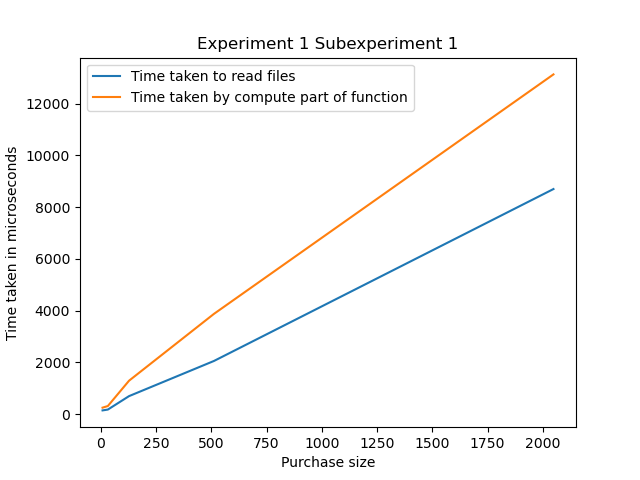
\includegraphics[width=1\textwidth]{exp1graphsubexp1.png}
\end{figure}
As everything is constant, the graph is clearly linear.\\ \newpage
\textbf{Subexperiment 2}:\\
\begin{itemize}
    \item No of unique products = 5
    \item No of hashtags per product = 4
    \item Total unique hashtags = 10
    \item No of customers = 6
\end{itemize}
I varied number of purchases between 8 to 2048 to get the following graph:
\begin{figure}[h]
    \centering
    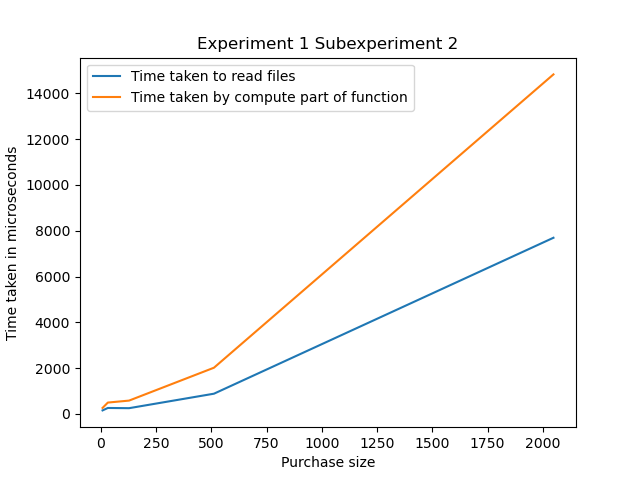
\includegraphics[width=1\textwidth]{exp1graphsubexp2.png}
\end{figure}
At lower purchases the other terms of the complexity are dominating such as the $O(pur*pd*h*(log(c) + pd*h/c))$ term, but after a point it becomes linear with purchases as it dominates.\\ \newpage
\textbf{Subexperiment 3}:\\
\begin{itemize}
    \item No of unique products = 10
    \item No of hashtags per product = 2
    \item Total unique hashtags = 10
    \item No of customers = 8
\end{itemize}
I varied number of purchases between 8 to 2048 to get the following graph:
\begin{figure}[h]
    \centering
    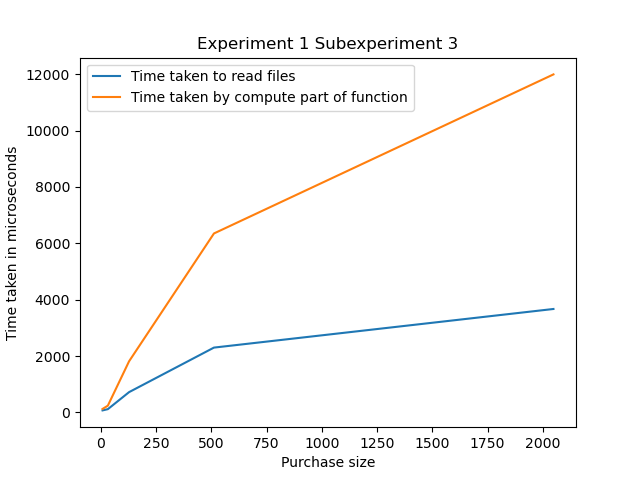
\includegraphics[width=1\textwidth]{exp1graphsubexp3.png}
\end{figure}
At lower purchases the other terms of the complexity are dominating, but after a point it becomes linear with purchases as it dominates.\\ \newpage
\textbf{Subexperiment 4}:\\
\begin{itemize}
    \item No of unique products = 10
    \item No of hashtags per product = 4
    \item Total unique hashtags = 10
    \item No of customers = 6
\end{itemize}
I varied number of purchases between 8 to 2048 to get the following graph:
\begin{figure}[h]
    \centering
    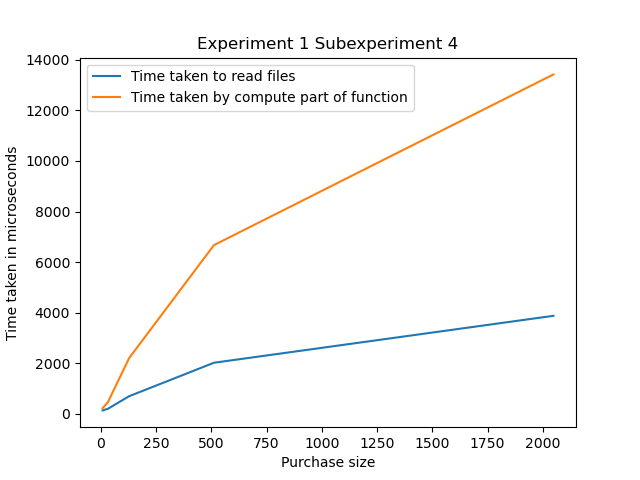
\includegraphics[width=1\textwidth]{exp1graphsubexp4.png}
\end{figure}
This graph has almost 3 segments, as the number of purchases is less, the $pd*h*c*\log(pd*h/c)$ term dominates until a point, when it is taken over by the purchase term which makes the linear.\\
\newpage
\textbf{Experiment 2}:\\
\textbf{Subexperiment 1}:\\
\begin{itemize}
    \item No of unique products = 5
    \item No of hashtags per product = 2
    \item Total unique hashtags = 10
    \item Here I have varied the number of customers between 4 to 64 to get the following graphs.
\end{itemize}
I vary the number of purchases between 8 to 2048 for each number of customers.\\
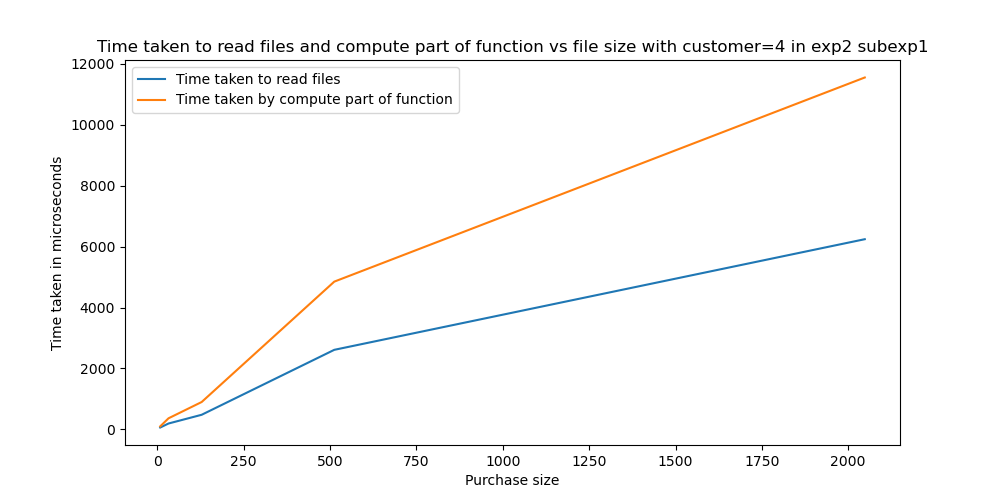
\includegraphics[width=1\textwidth]{exp2graphsubexp1customer4.png}
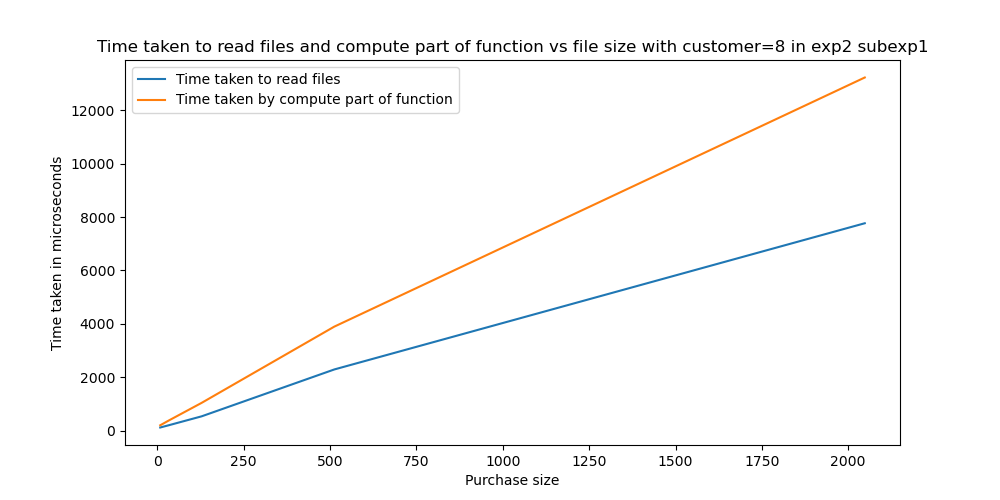
\includegraphics[width=1\textwidth]{exp2graphsubexp1customer8.png}
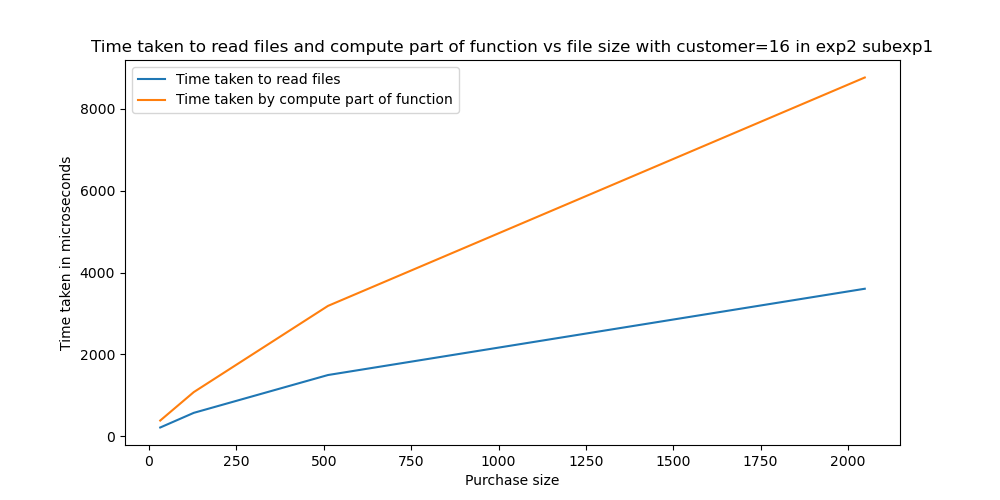
\includegraphics[width=1\textwidth]{exp2graphsubexp1customer16.png}
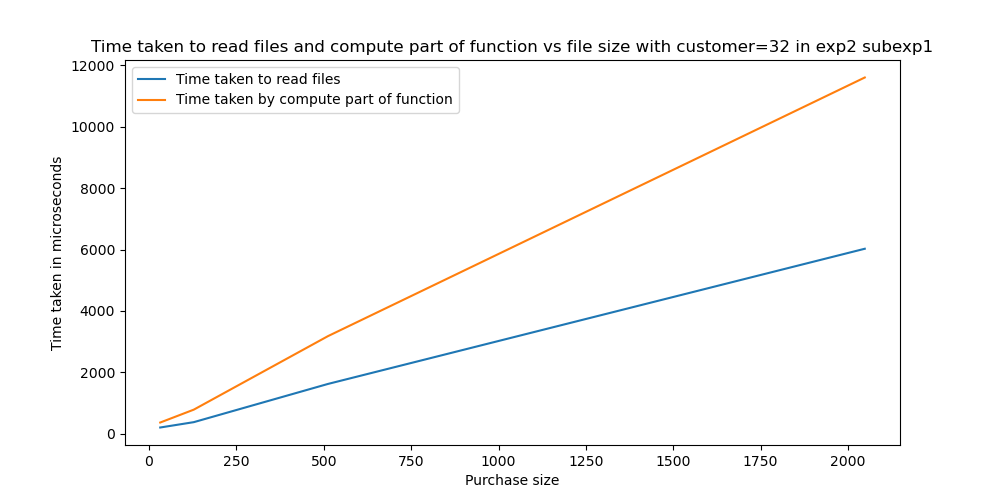
\includegraphics[width=1\textwidth]{exp2graphsubexp1customer32.png}
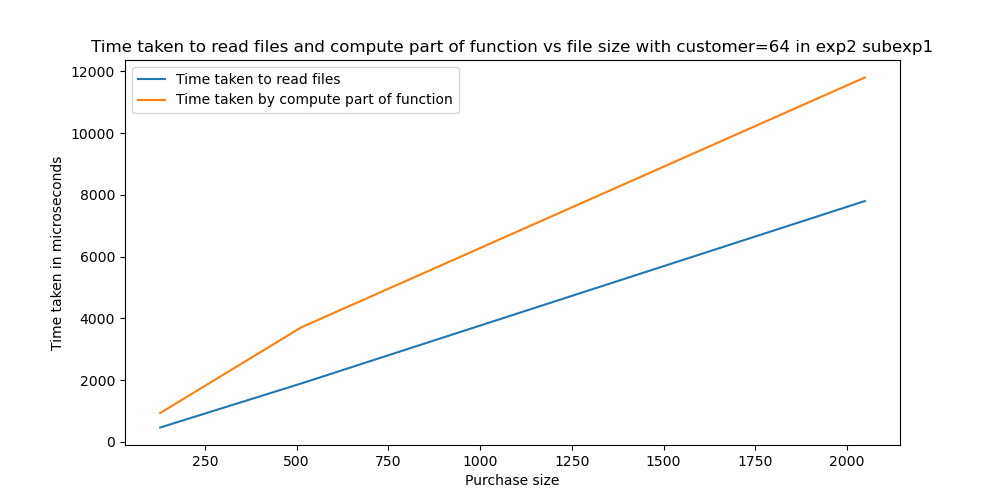
\includegraphics[width=1\textwidth]{exp2graphsubexp1customer64.png}\\
As we can see from these graphs for a constant number of products, hashtags per product, and customers, the time complexity is linear with the purchases. The times vary slightly with the number of customers, most likely due to the $O(c*\log(c))$ term.\\
I have also compared the time complexity for a constant number of purchases and products, but varying the number of customers.\\
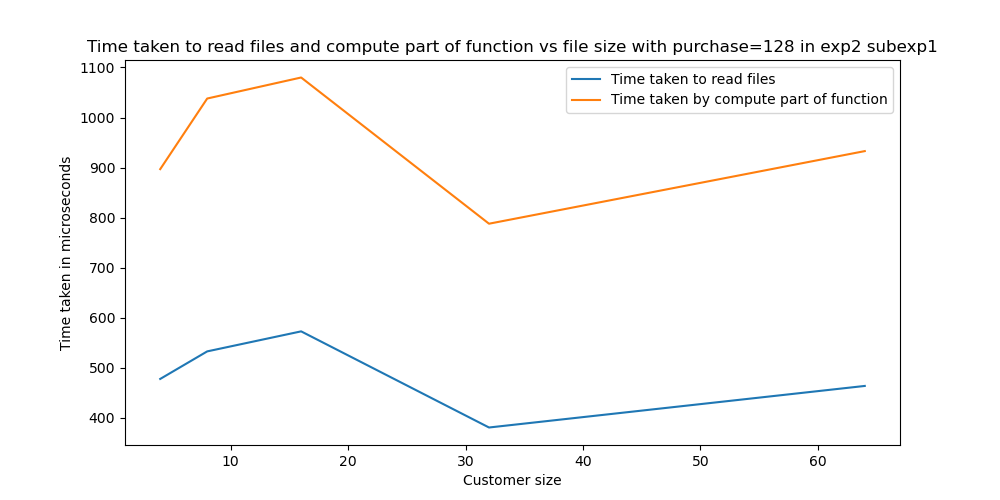
\includegraphics[width=1\textwidth]{exp2graphsubexp1purchase128.png}
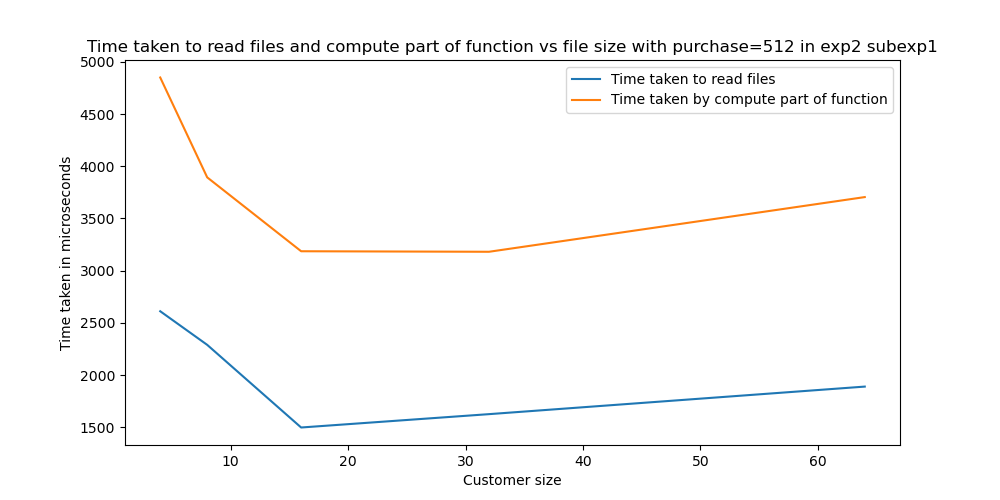
\includegraphics[width=1\textwidth]{exp2graphsubexp1purchase512.png}
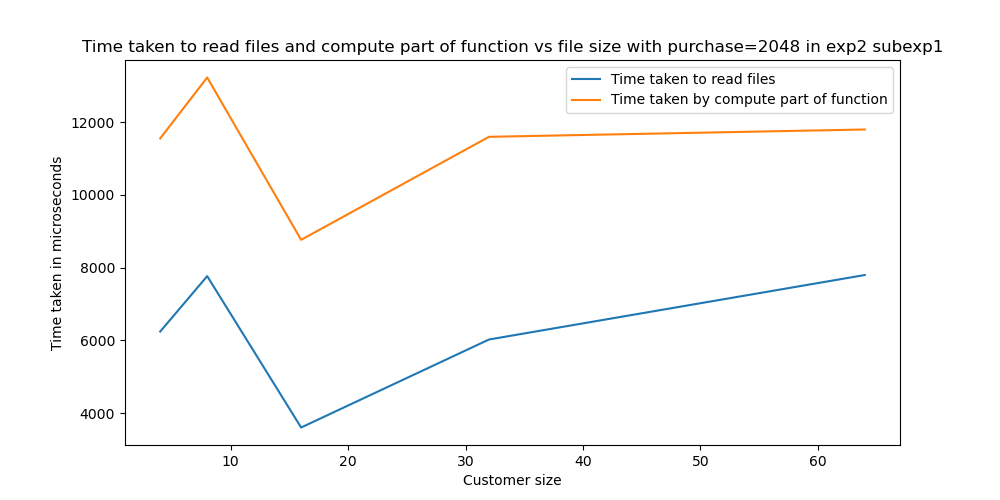
\includegraphics[width=1\textwidth]{exp2graphsubexp1purchase2048.png}\\
This is a mismatch of complexities as the c term is present in multiple terms of the complexity term. Hence we see a pathwork of complexities as c varies and starts to dominate.\\
But we can clearly see that as number of purchases increase, the time taken on average increases, which is expected.\\

\textbf{Subexperiment 2}:\\
\begin{itemize}
    \item No of unique products = 5
    \item No of hashtags per product = 4
    \item Total unique hashtags = 10
    \item Here I have varied the number of customers between 4 to 64 to get the following graphs.
\end{itemize}
I vary the number of purchases between 8 to 2048 for each number of customers.\\
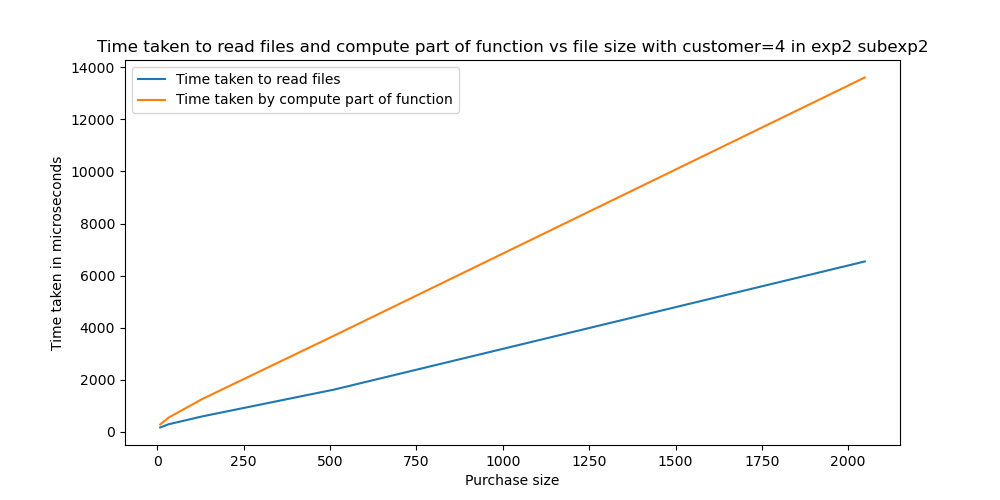
\includegraphics[width=1\textwidth]{exp2graphsubexp2customer4.png}
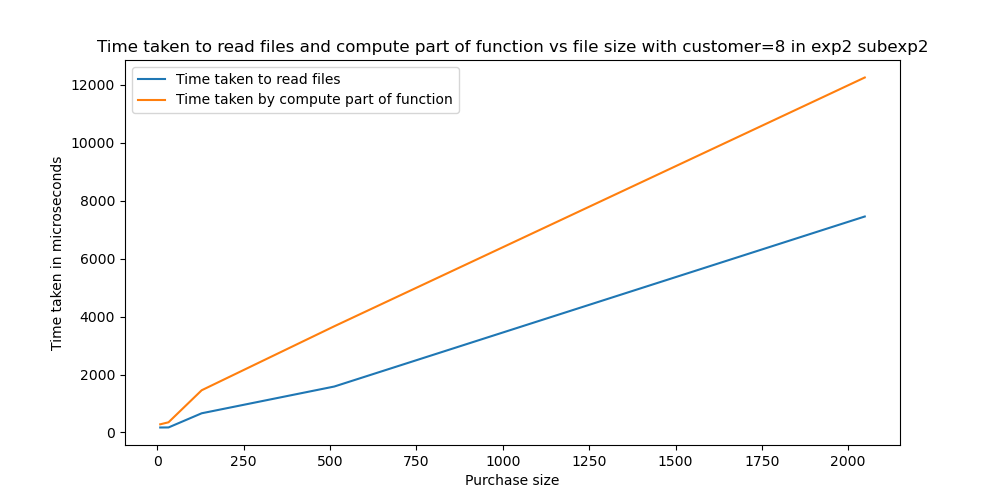
\includegraphics[width=1\textwidth]{exp2graphsubexp2customer8.png}
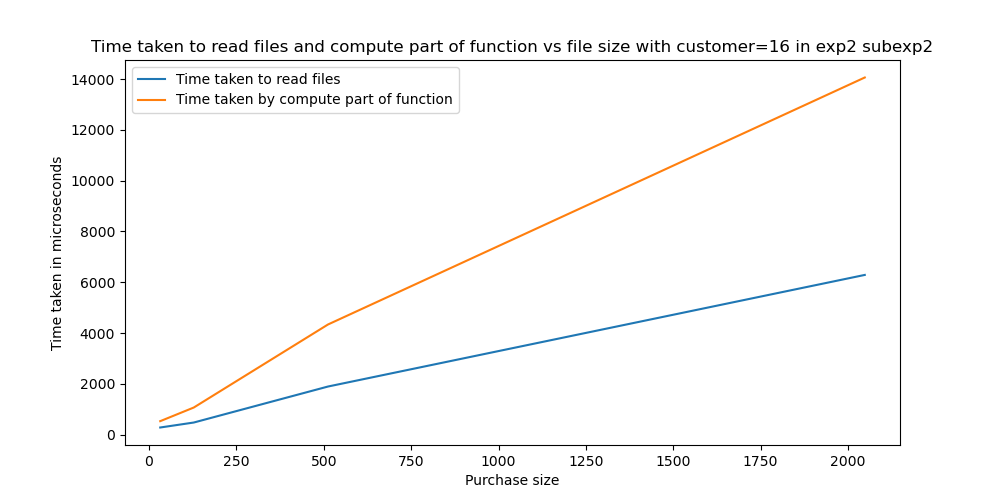
\includegraphics[width=1\textwidth]{exp2graphsubexp2customer16.png}
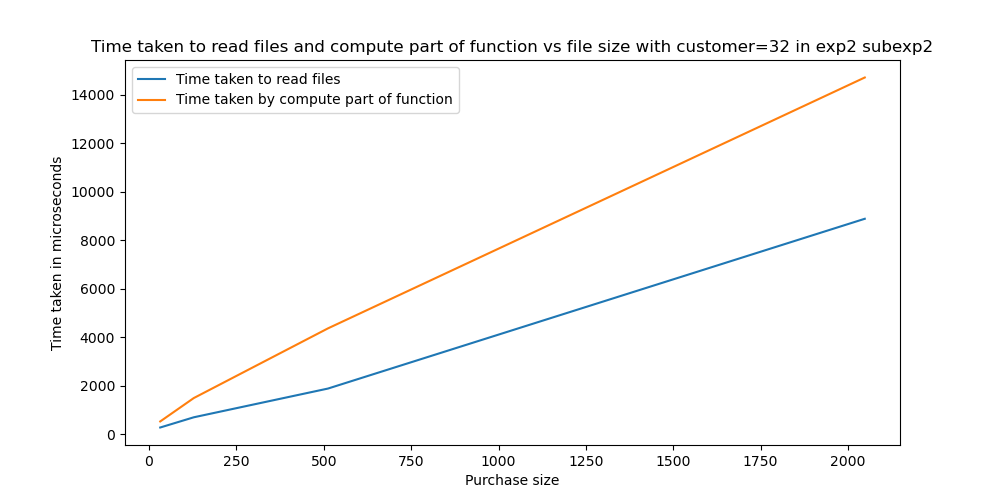
\includegraphics[width=1\textwidth]{exp2graphsubexp2customer32.png}
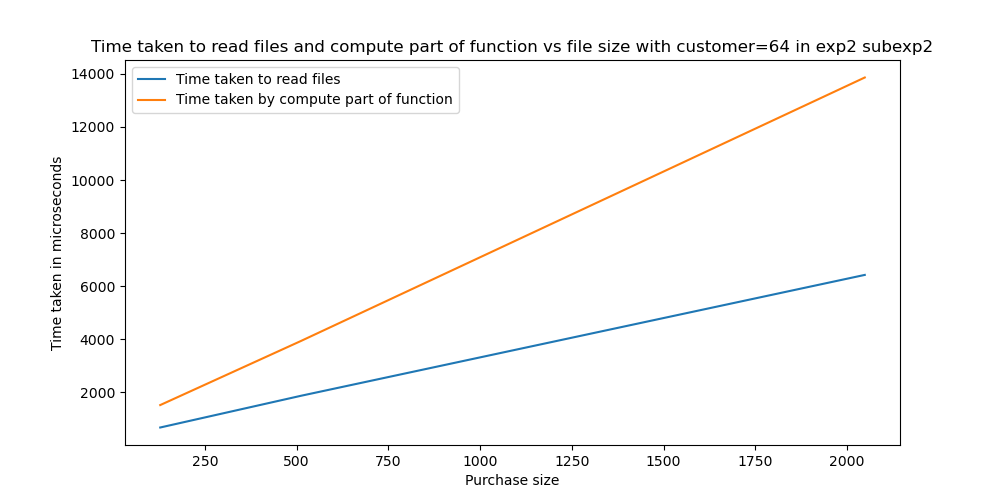
\includegraphics[width=1\textwidth]{exp2graphsubexp2customer64.png}\\
As we can see from these graphs for a constant number of products, hashtags per product, and customers, the time complexity is linear with the purchases. The times vary slightly with the number of customers, most likely due to the $O(c*\log(c))$ term.\\
I have also compared the time complexity for a constant number of purchases and products, but varying the number of customers.\\
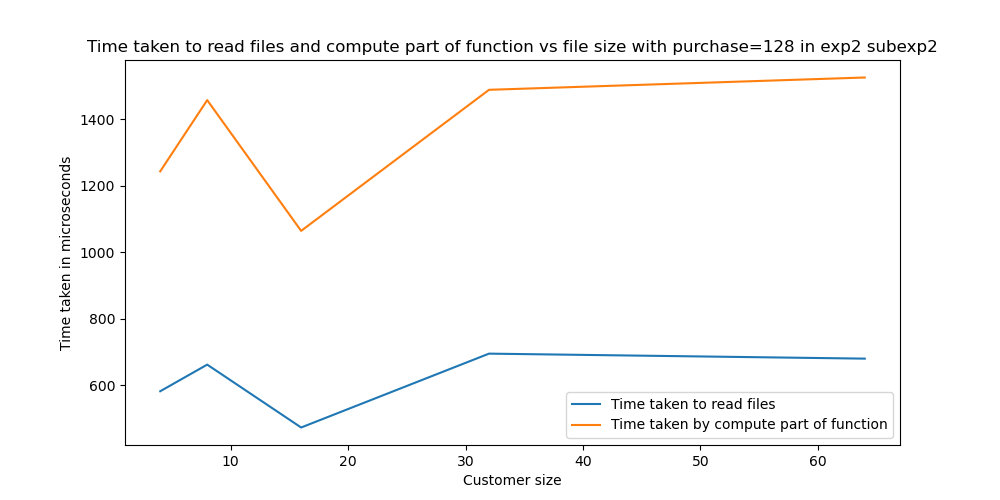
\includegraphics[width=1\textwidth]{exp2graphsubexp2purchase128.png}
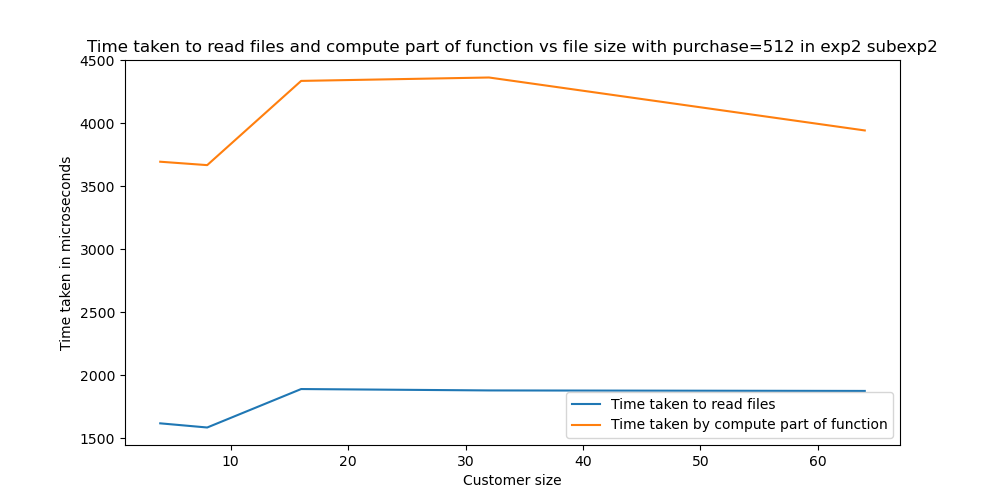
\includegraphics[width=1\textwidth]{exp2graphsubexp2purchase512.png}
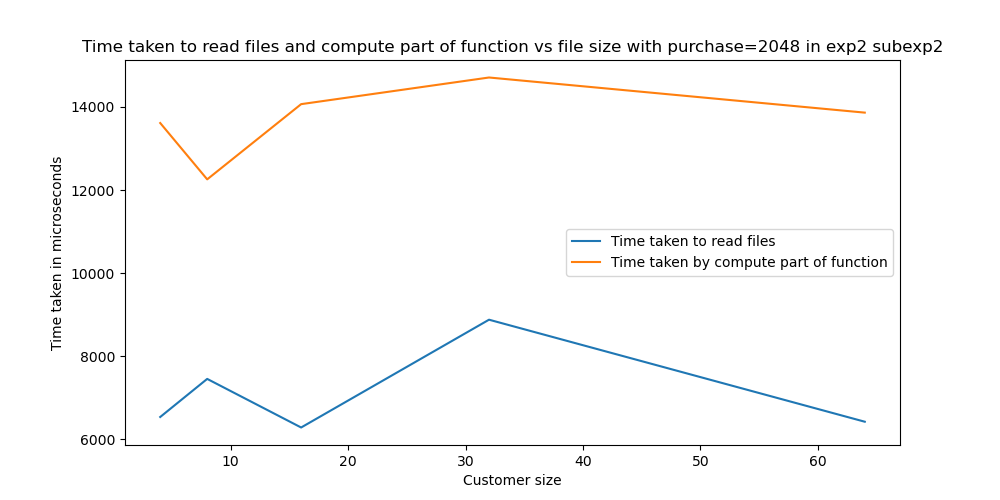
\includegraphics[width=1\textwidth]{exp2graphsubexp2purchase2048.png}\\
This is a mismatch of complexities as the c term is present in multiple terms of the complexity term. Hence we see a patchwork of complexities as c varies and starts to dominate.\\
But we can clearly see that as number of purchases increase, the time taken on average increases, which is expected.\\

\textbf{Subexperiment 3}:\\
\begin{itemize}
    \item No of unique products = 10
    \item No of hashtags per product = 2
    \item Total unique hashtags = 10
    \item Here I have varied the number of customers between 4 to 64 to get the following graphs.
\end{itemize}
I vary the number of purchases between 8 to 2048 for each number of customers.\\
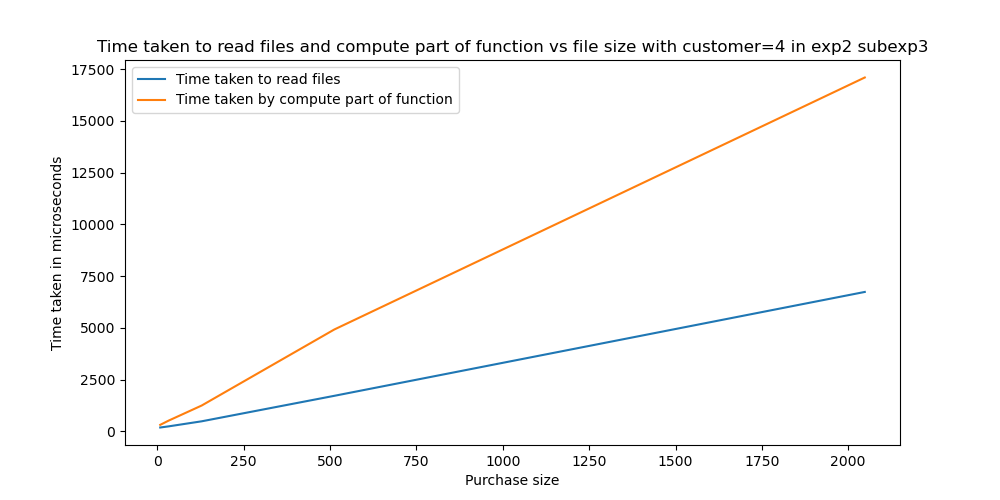
\includegraphics[width=1\textwidth]{exp2graphsubexp3customer4.png}
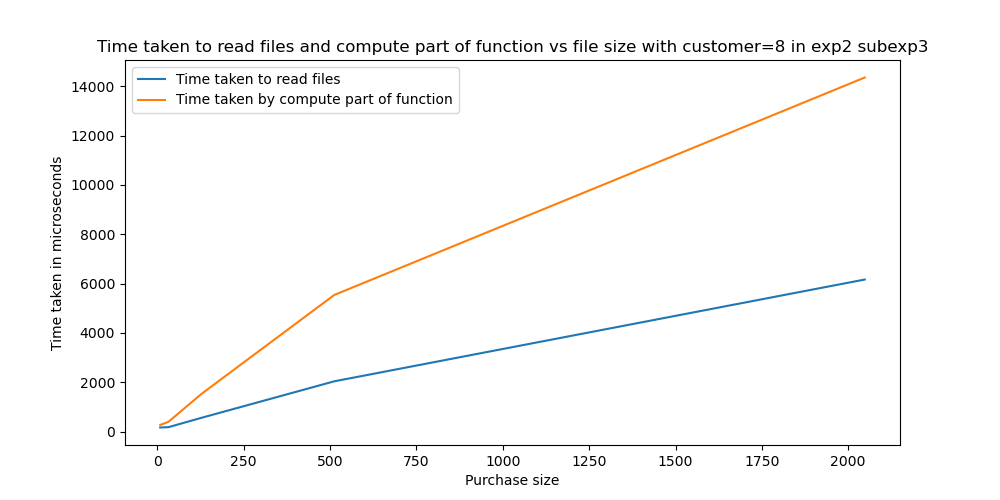
\includegraphics[width=1\textwidth]{exp2graphsubexp3customer8.png}
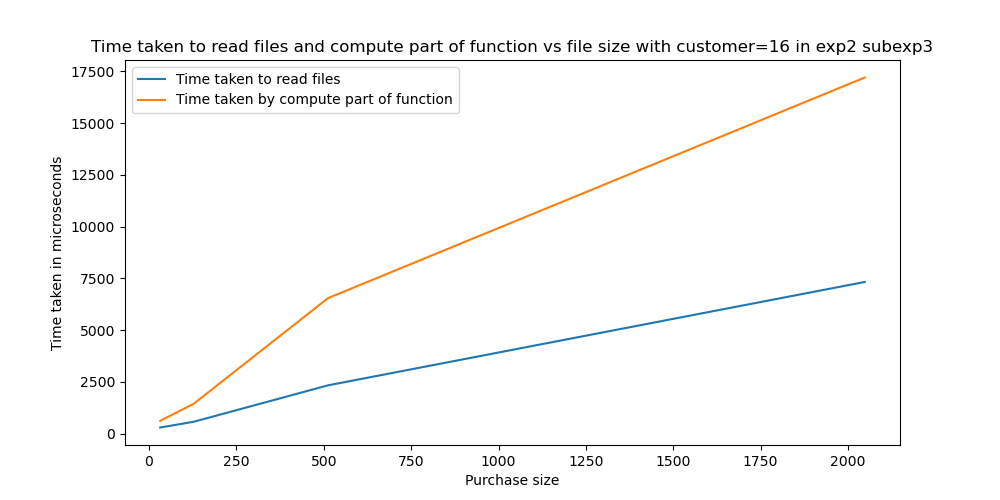
\includegraphics[width=1\textwidth]{exp2graphsubexp3customer16.png}
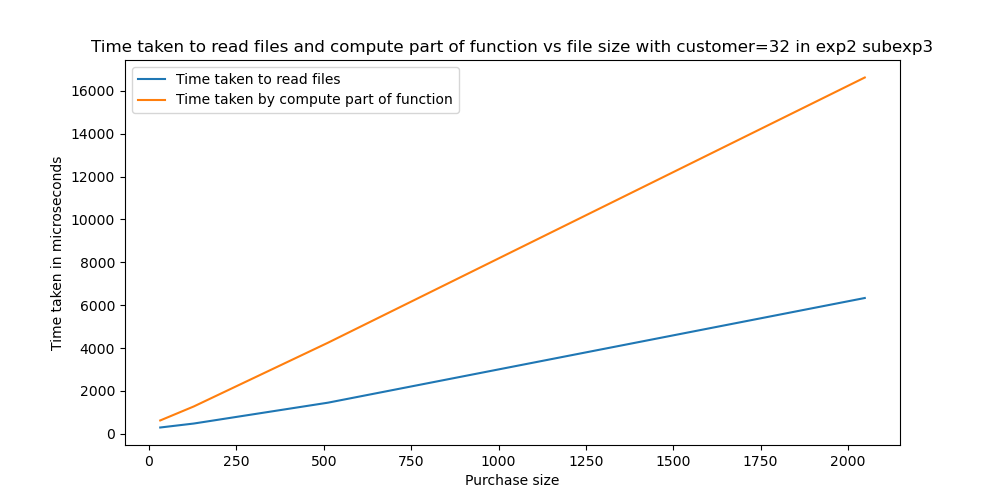
\includegraphics[width=1\textwidth]{exp2graphsubexp3customer32.png}
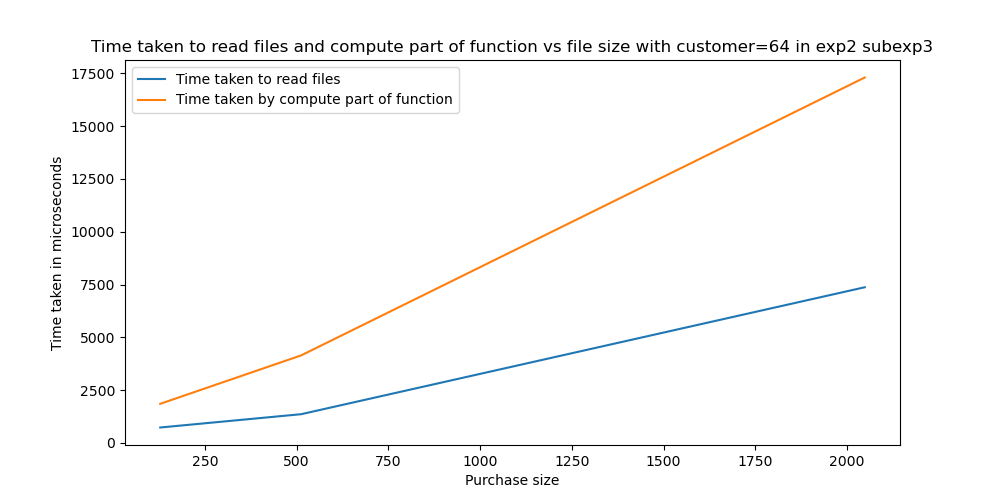
\includegraphics[width=1\textwidth]{exp2graphsubexp3customer64.png}\\
As we can see from these graphs for a constant number of products, hashtags per product, and customers, the time complexity is linear with the purchases. The times vary slightly with the number of customers, most likely due to the $O(c*\log(c))$ term.\\
I have also compared the time complexity for a constant number of purchases and products, but varying the number of customers.\\
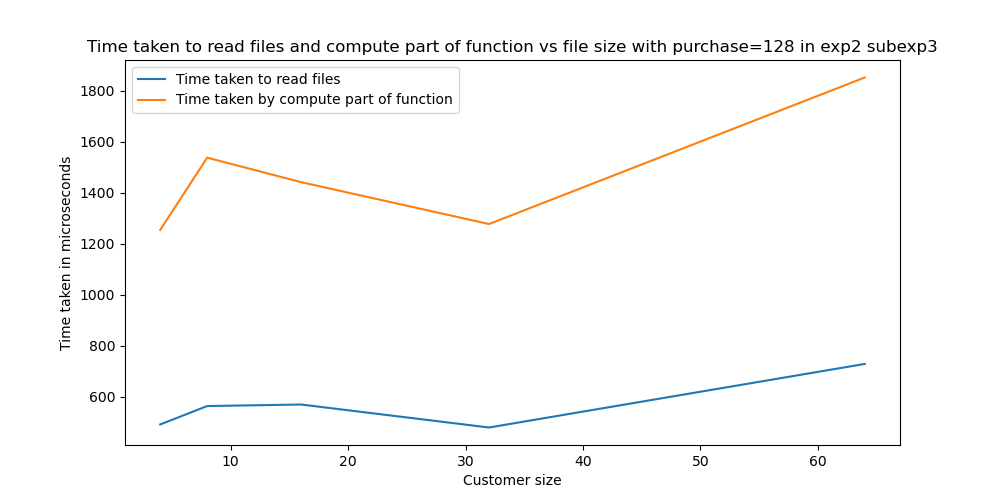
\includegraphics[width=1\textwidth]{exp2graphsubexp3purchase128.png}
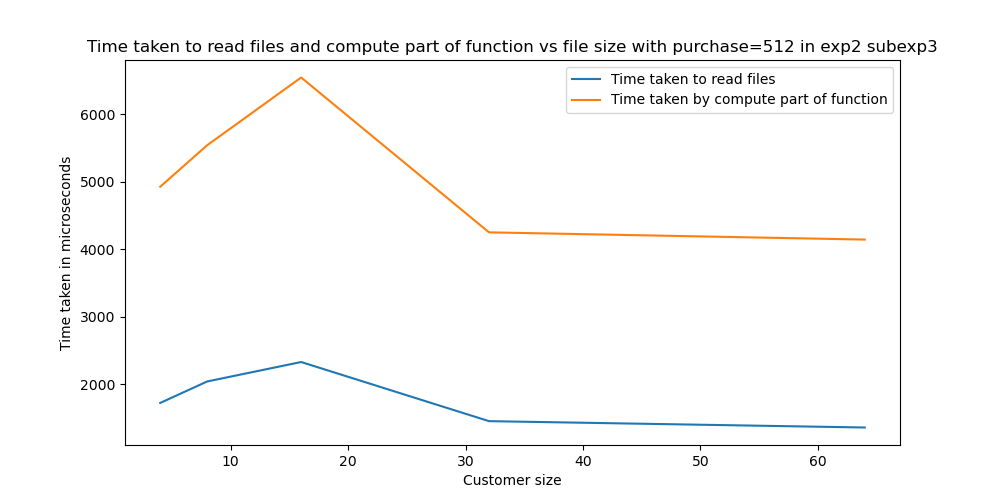
\includegraphics[width=1\textwidth]{exp2graphsubexp3purchase512.png}
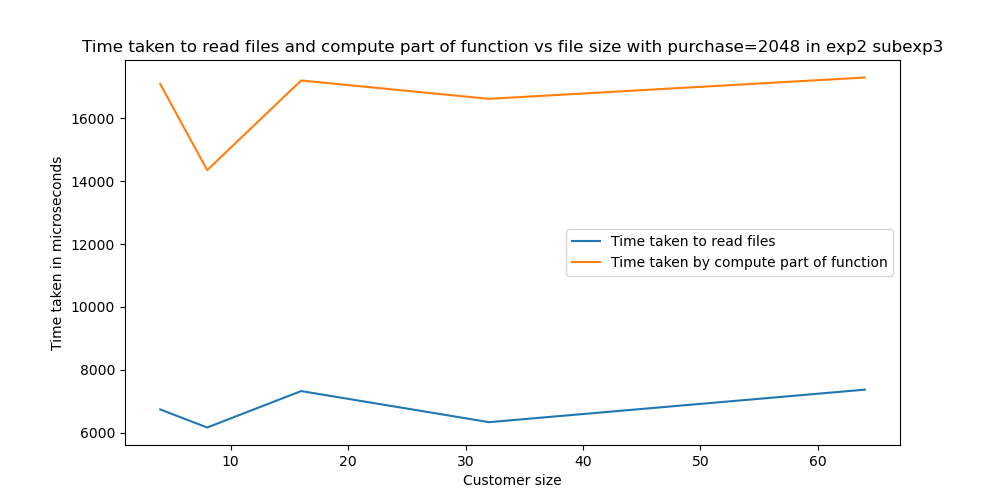
\includegraphics[width=1\textwidth]{exp2graphsubexp3purchase2048.png}\\
This is a mismatch of complexities as the c term is present in multiple terms of the complexity term. Hence we see a patchwork of complexities as c varies and starts to dominate.\\
But we can clearly see that as number of purchases increase, the time taken on average increases, which is expected.\\

\textbf{Subexperiment 4}:\\
\begin{itemize}
    \item No of unique products = 10
    \item No of hashtags per product = 4
    \item Total unique hashtags = 10
    \item Here I have varied the number of customers between 4 to 64 to get the following graphs.
\end{itemize}
I vary the number of purchases between 8 to 2048 for each number of customers.\\
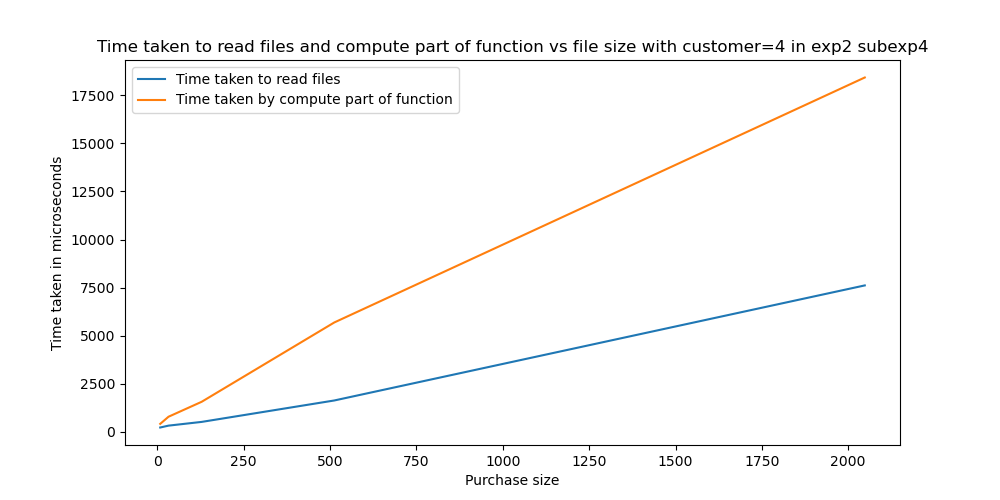
\includegraphics[width=1\textwidth]{exp2graphsubexp4customer4.png}
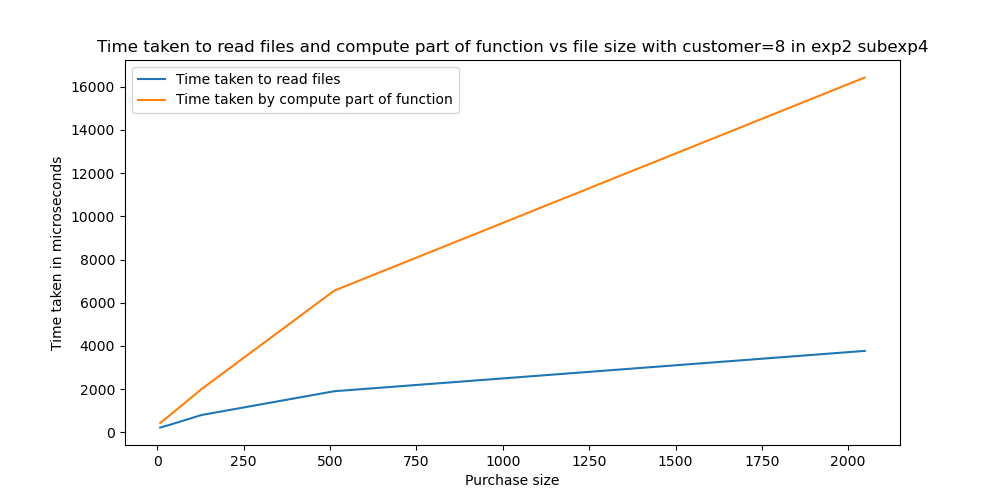
\includegraphics[width=1\textwidth]{exp2graphsubexp4customer8.png}
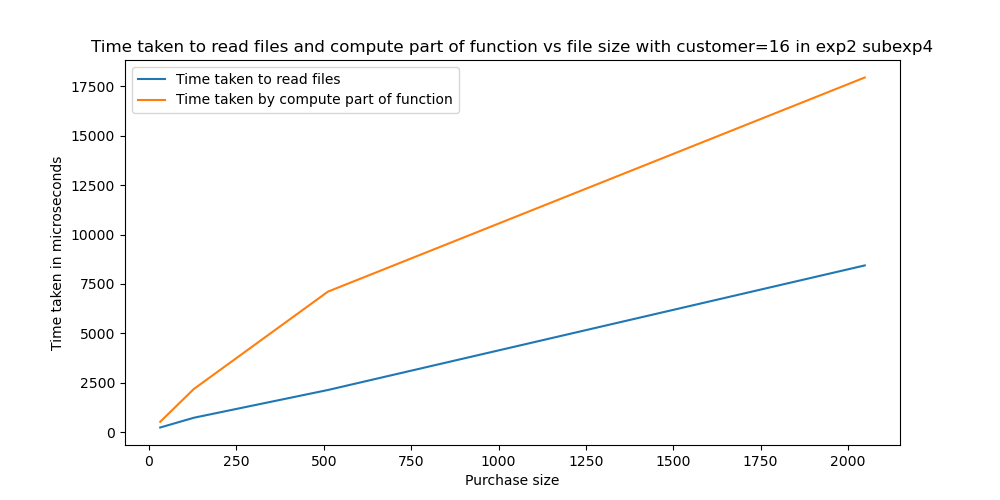
\includegraphics[width=1\textwidth]{exp2graphsubexp4customer16.png}
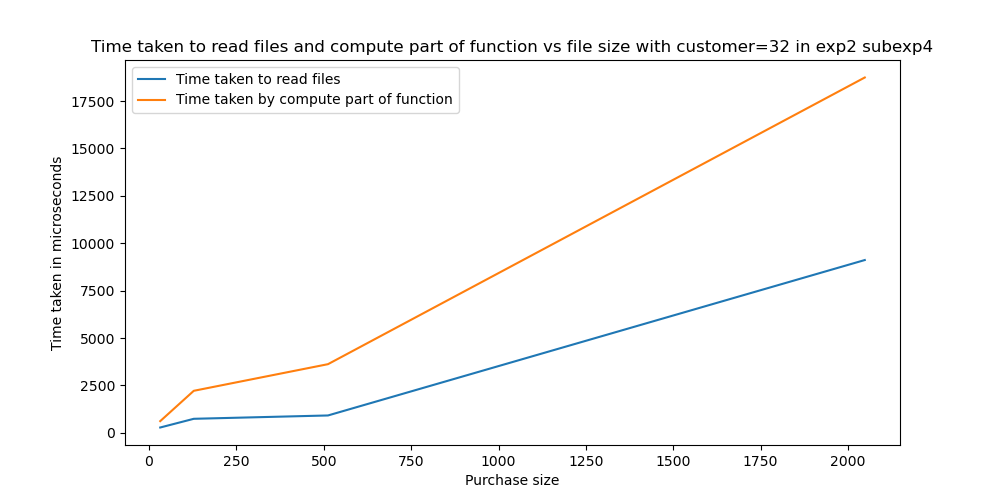
\includegraphics[width=1\textwidth]{exp2graphsubexp4customer32.png}
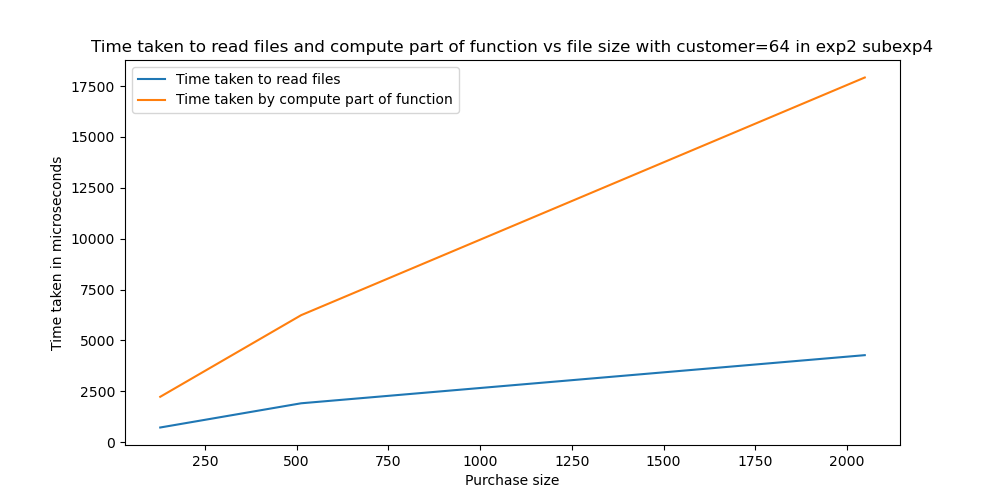
\includegraphics[width=1\textwidth]{exp2graphsubexp4customer64.png}\\
As we can see from these graphs for a constant number of products, hashtags per product, and customers, the time complexity is linear with the purchases. The times vary slightly with the number of customers, most likely due to the $O(c*\log(c))$ term.\\
I have also compared the time complexity for a constant number of purchases and products, but varying the number of customers.\\
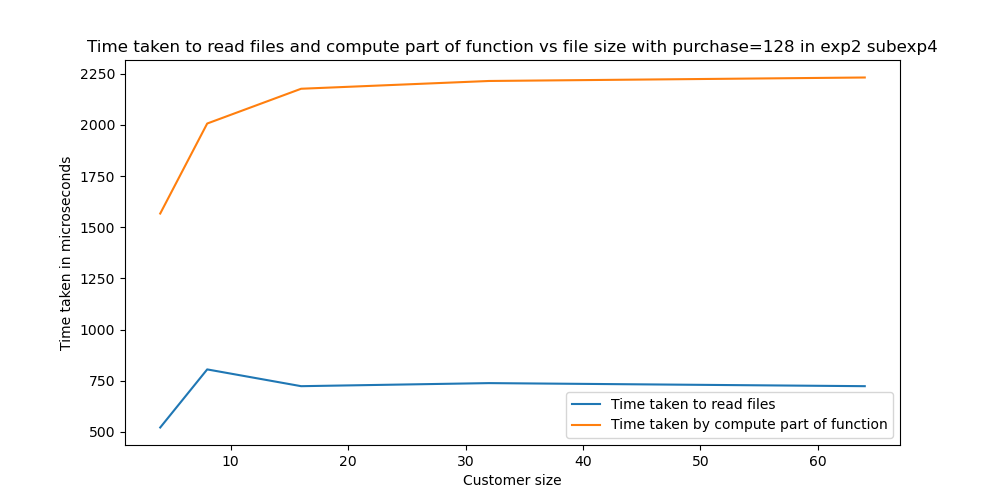
\includegraphics[width=1\textwidth]{exp2graphsubexp4purchase128.png}
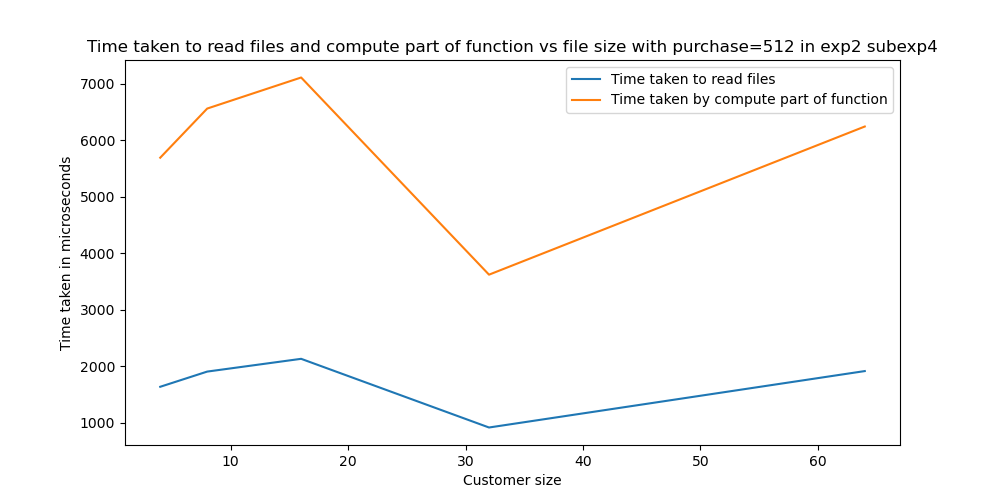
\includegraphics[width=1\textwidth]{exp2graphsubexp4purchase512.png}
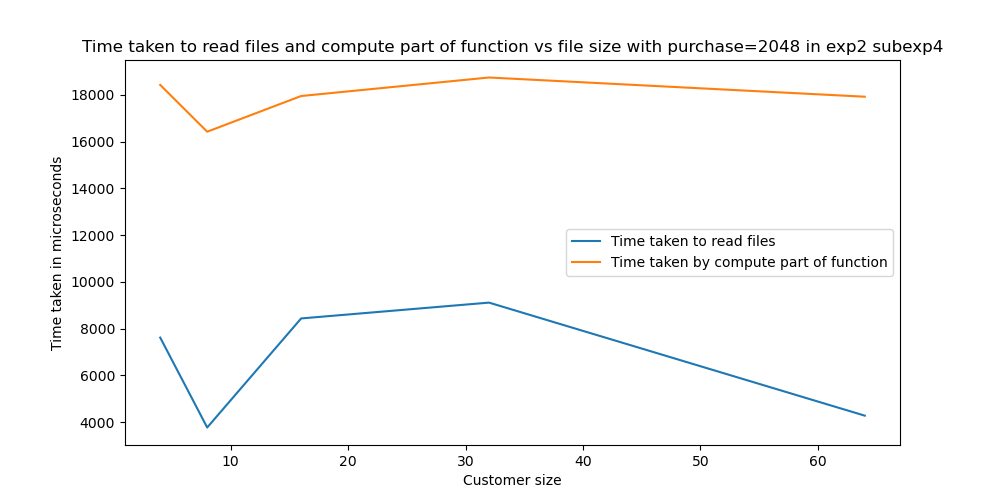
\includegraphics[width=1\textwidth]{exp2graphsubexp4purchase2048.png}\\
This is a mismatch of complexities as the c term is present in multiple terms of the complexity term. Hence we see a patchwork of complexities as c varies and starts to dominate.\\
But we can clearly see that as number of purchases increase, the time taken on average increases, which is expected.\\

\textbf{Experiment 3-5}:\\
I randomized the number of hashtags per product, and ran the same experiments as done in experiment 2. The results were similar to the ones obtained in experiment 2.\\
\textbf{Subexperiment 1}:\\
\begin{itemize}
    \item No of unique products = 5
    \item Total unique hashtags = 10
\end{itemize}
As the experiments I conducted are extensive, I will only show some sample graphs from here.\\
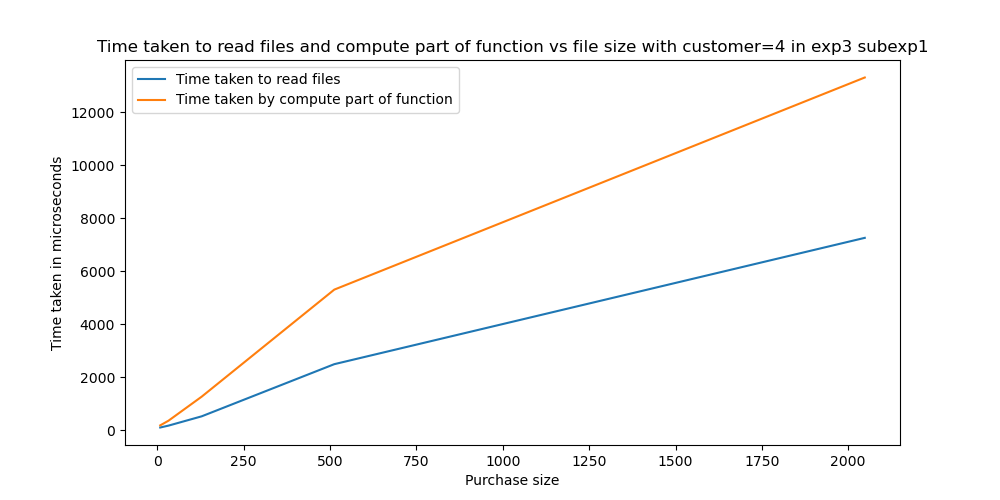
\includegraphics[width=1\textwidth]{exp3graphsubexp1customer4.png}  
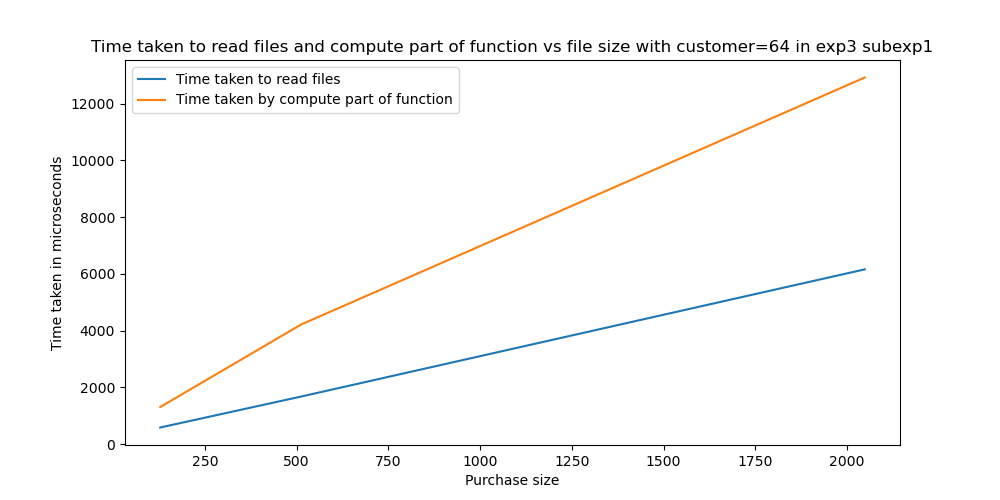
\includegraphics[width=1\textwidth]{exp3graphsubexp1customer64.png}
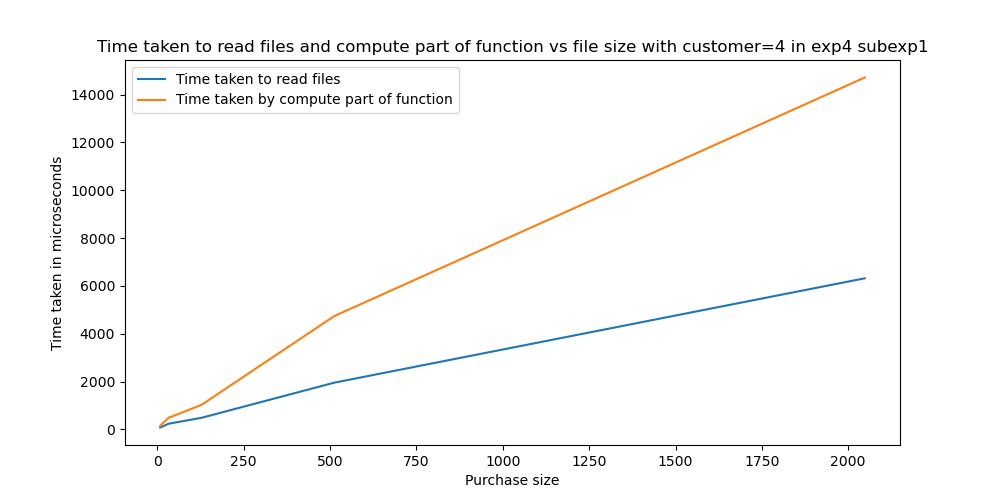
\includegraphics[width=1\textwidth]{exp4graphsubexp1customer4.png}  
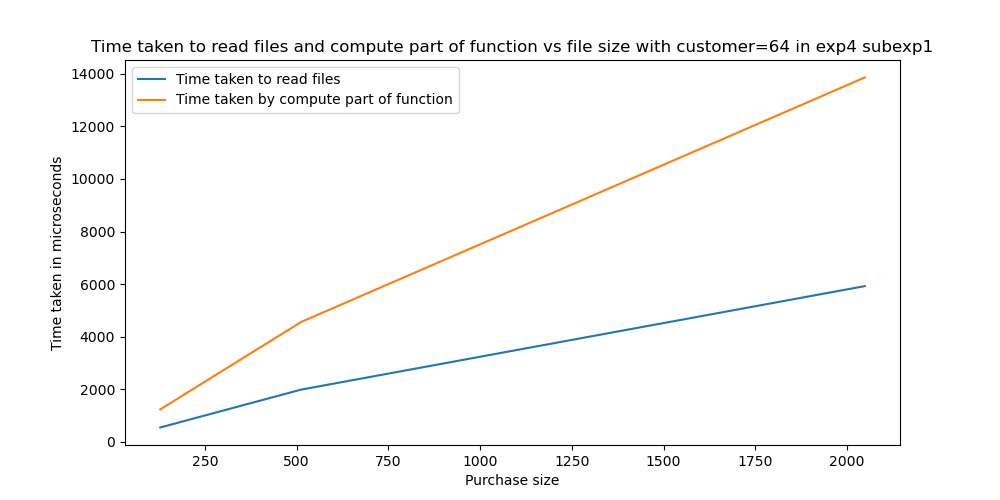
\includegraphics[width=1\textwidth]{exp4graphsubexp1customer64.png}
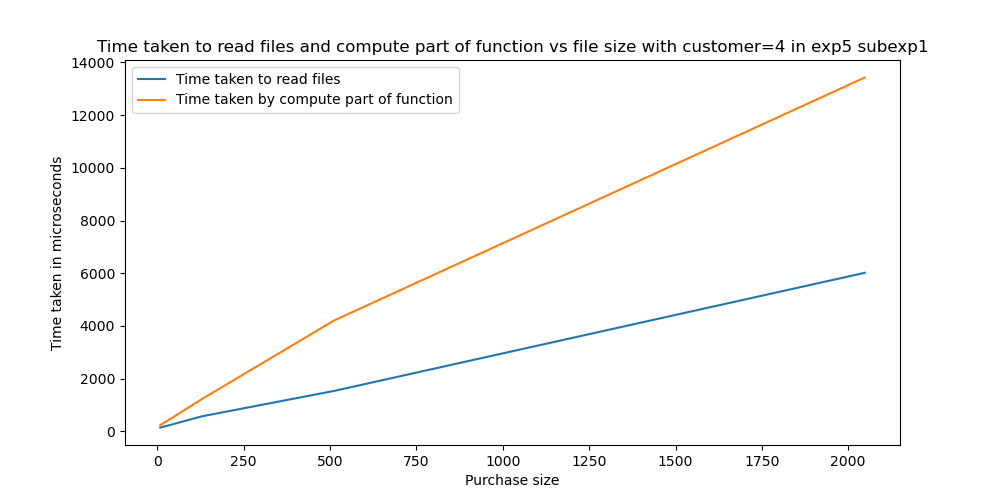
\includegraphics[width=1\textwidth]{exp5graphsubexp1customer4.png}  
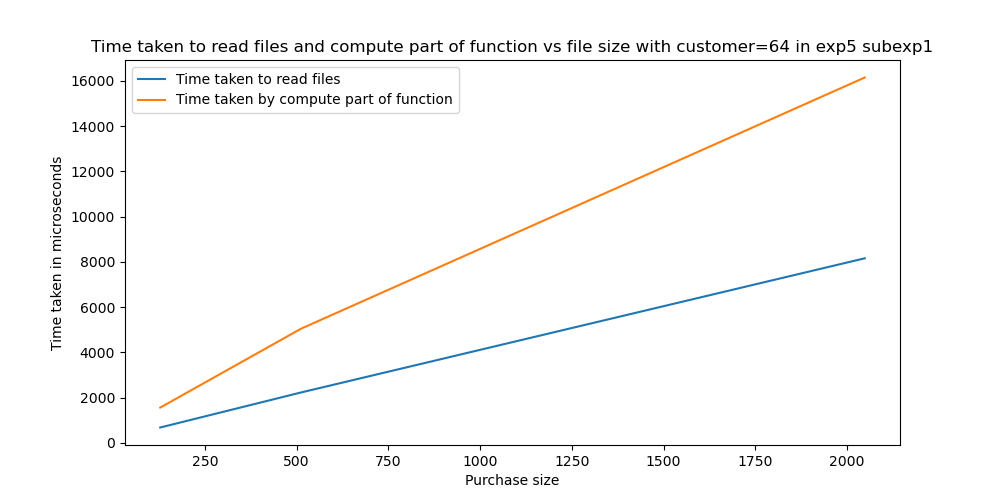
\includegraphics[width=1\textwidth]{exp5graphsubexp1customer64.png}\\

The time taken for each exp increases form subexp1 to subexp3 as the number of customers increase.\\

\textbf{Subexperiment 2}:\\
\begin{itemize}
    \item No of unique products = 10
    \item Total unique hashtags = 10
\end{itemize}

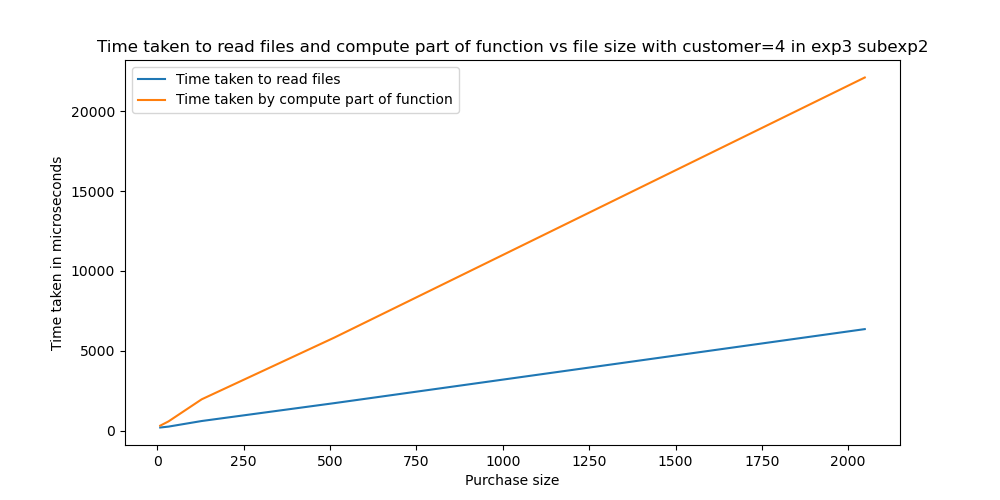
\includegraphics[width=1\textwidth]{exp3graphsubexp2customer4.png}
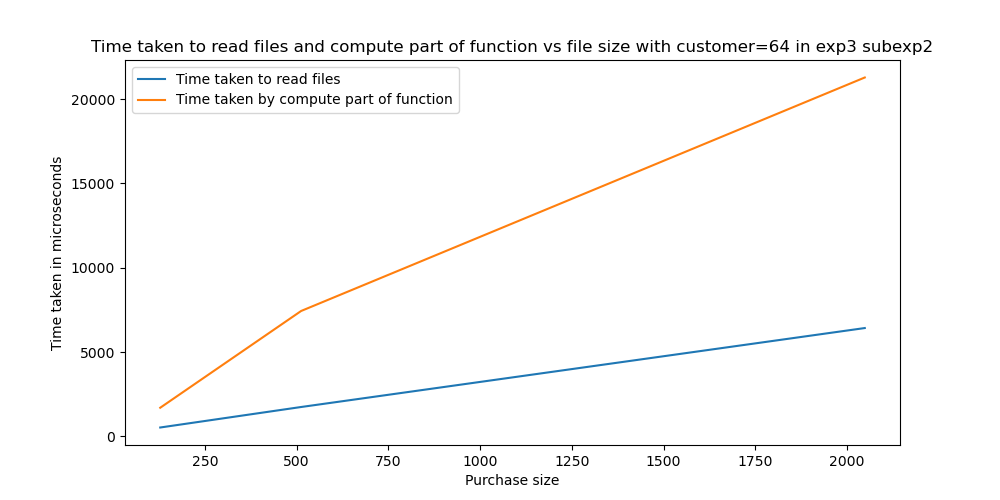
\includegraphics[width=1\textwidth]{exp3graphsubexp2customer64.png}
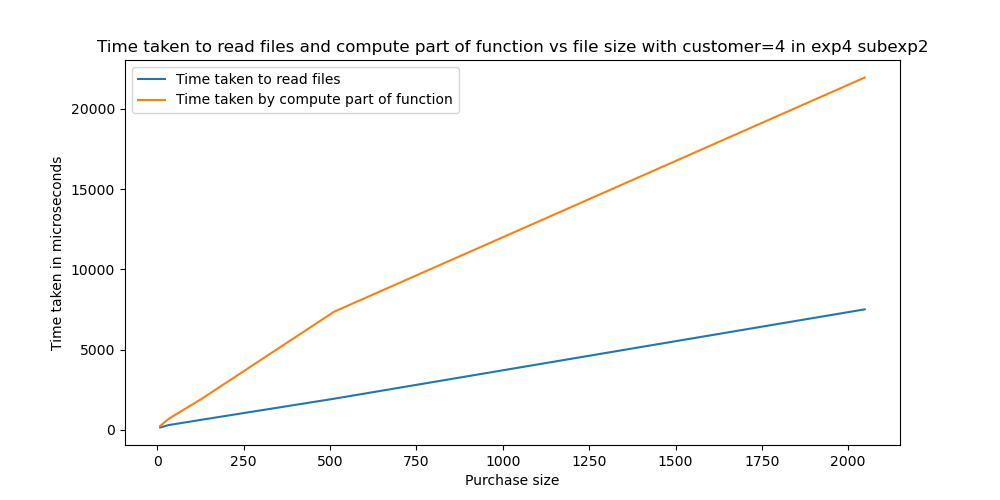
\includegraphics[width=1\textwidth]{exp4graphsubexp2customer4.png}
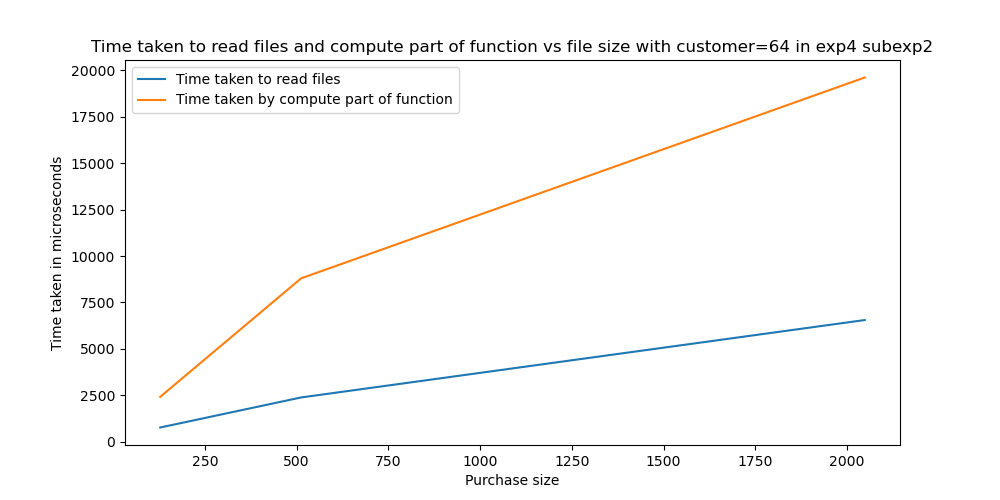
\includegraphics[width=1\textwidth]{exp4graphsubexp2customer64.png}
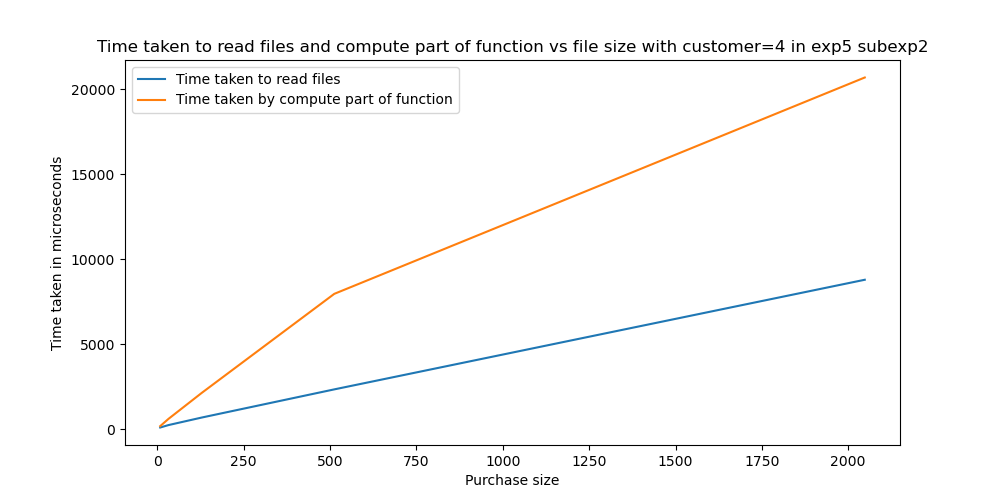
\includegraphics[width=1\textwidth]{exp5graphsubexp2customer4.png}
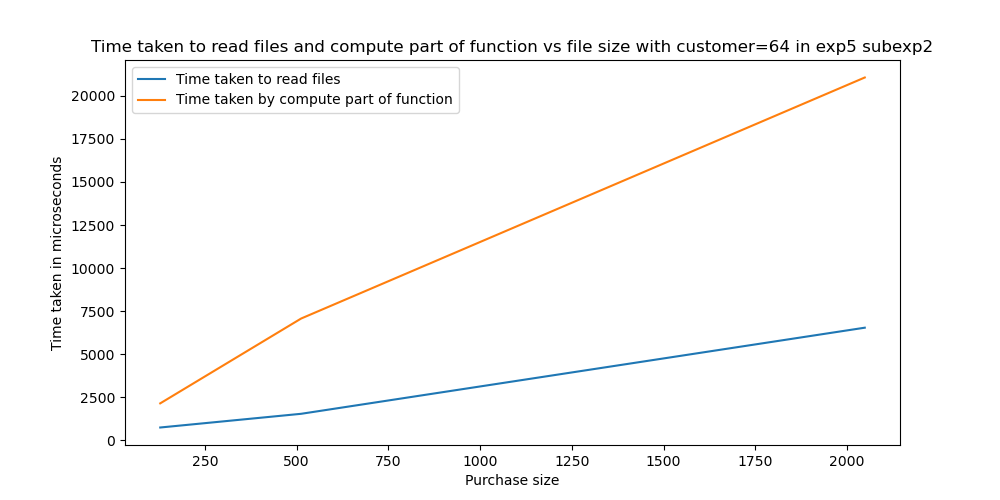
\includegraphics[width=1\textwidth]{exp5graphsubexp2customer64.png}\\

The time taken for each exp increases form subexp1 to subexp3 as the number of customers increase.\\

\textbf{Subexperiment 3}:\\
\begin{itemize}
    \item No of unique products = 20
    \item Total unique hashtags = 10
\end{itemize}

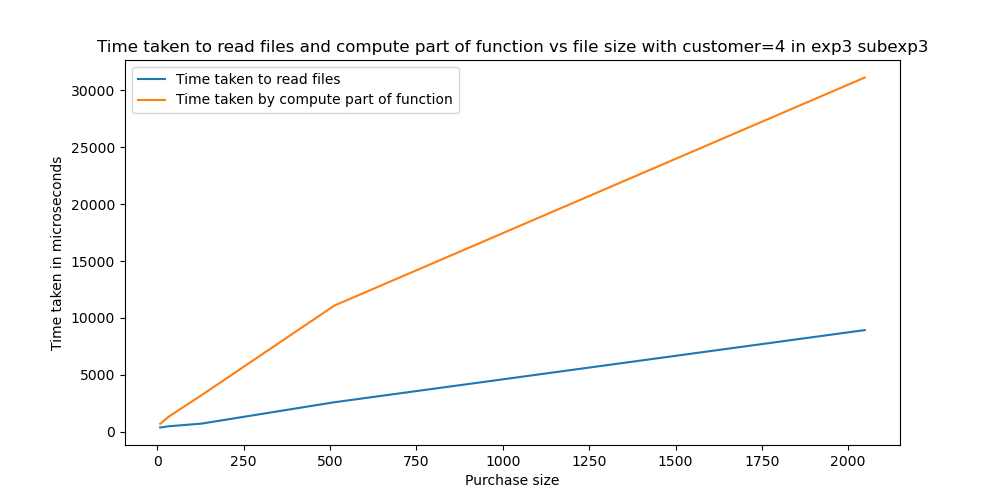
\includegraphics[width=1\textwidth]{exp3graphsubexp3customer4.png}
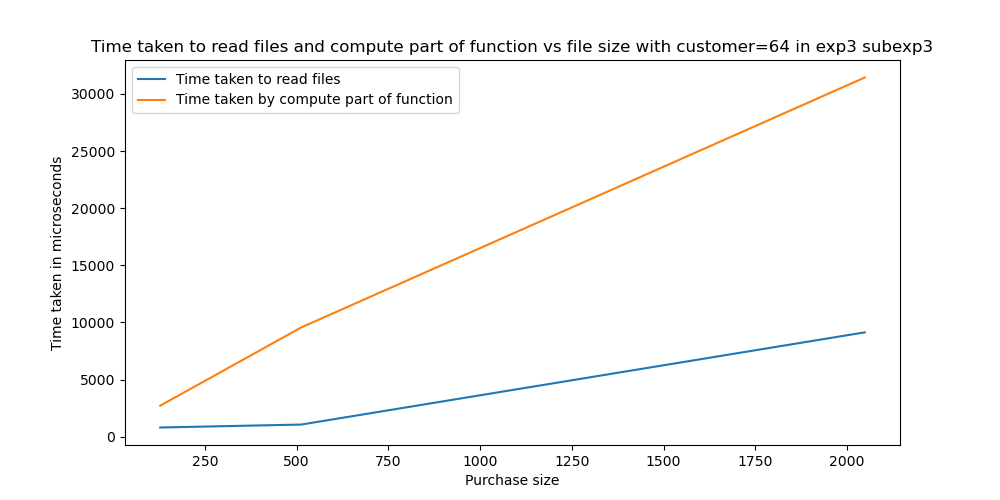
\includegraphics[width=1\textwidth]{exp3graphsubexp3customer64.png}
\includegraphics[width=1\textwidth]{exp4graphsubexp3customer4.png}
\includegraphics[width=1\textwidth]{exp4graphsubexp3customer64.png}
\includegraphics[width=1\textwidth]{exp5graphsubexp3customer4.png}
\includegraphics[width=1\textwidth]{exp5graphsubexp3customer64.png}\\

The time taken for exp increases form subexp1 to subexp3 as the number of customers increase.\\

\textbf{Observations:}\\
Overall, as the number of unique products increase, the time taken increases accross each experiment, as seen in the graphs. Each graph verifies the time complexity.\\

\textbf{Time Complexity of Writing the groups to the output:}\\
Unfortunately, I was unable to measure this time complexity empirically, as in the code the $fileIO$ variable was taken as 0 for all experiments that I was running. After looking into this for a while, I found out that beacuse C++ is so efficient, it caches the outputs and since the files are writing to the same output files, it is just skipping this operation altogether, hence making it 0. Thus for all my experiments the time taken by funciton and total time taken are the same. I have tried running this on my own system to see if there was any change, but the results were the same. Hence I chalk this up to a language specific feature of c++ and do not report any reults here.\\

\textbf{Space Complexity Analysis:}\\
Throughout my code, I use vectors and maps. The space complexity for the code is as follows:
\begin{itemize}
    \item productHashtags: $O(pd*h)$
    \item customerPurchases: $O(pur)$
    \item customerHashtags: $O(c*pd*h)$
    \item customerTopKHashtags: $O(pd*h)$
    \item customerGroup: $O(c)$
\end{itemize}
The total space complexity is $O(pd*h + pur + c*pd*h + c)$.\\

To measure the space complexity, we use maximum resident size, printed to terminal. This is the maximum memory accessed by the program during its run time.\\
I have measured the space complexity for the code in \textbf{experiment 2} which has the following results:\\
\textbf{Subexperiment 1}:\\
\begin{itemize}
    \item No of unique products = 5
    \item No of hashtags per product = 2
\end{itemize}
I varied number of purchases between 8 to 2048 to get the following graphs:
\includegraphics[width=1\textwidth]{Memorysubexp1customer4mem.png}
\includegraphics[width=1\textwidth]{Memorysubexp1customer8mem.png}
\includegraphics[width=1\textwidth]{Memorysubexp1customer16mem.png}
\includegraphics[width=1\textwidth]{Memorysubexp1customer32mem.png}
\includegraphics[width=1\textwidth]{Memorysubexp1customer64mem.png}\\
Here as $pur$ increases, it becomes the dominating term, hence the graph is linear after a point.\\

\textbf{Subexperiment 2}:\\
\begin{itemize}
    \item No of unique products = 5
    \item No of hashtags per product = 4
\end{itemize}
I varied number of purchases between 8 to 2048 to get the following graphs:
\includegraphics[width=1\textwidth]{Memorysubexp2customer4mem.png}
\includegraphics[width=1\textwidth]{Memorysubexp2customer8mem.png}
\includegraphics[width=1\textwidth]{Memorysubexp2customer16mem.png}
\includegraphics[width=1\textwidth]{Memorysubexp2customer32mem.png}
\includegraphics[width=1\textwidth]{Memorysubexp2customer64mem.png}\\
Here as $pur$ increases, it becomes the dominating term, hence the graph is linear after a point.\\

The other two subexperiments also follow the same trends, hence I shall not show them here.\\

It is clear from the graphs that as the complexity increases, but as c++ is an efficient language, this doesn't differ too much from each case.\\

\section*{Question 2}
There was no analysis of question 2 asked of me. The written code is in $user\_code.h$ file.\\

\section*{Question 3}
The optimized grouping function is as follows:
\begin{verbatim}
    if(!globalproductHashtagsInitialized){
        // #PROMPT# Extract all the lines from the hashtags 
        file and store them in an appropriate data structure
        vector<pair<string,vector<string>>> productHashtags;
        while(hashtags.hasNext()){
            string line = hashtags.next();
            vector<string> tokens = split(line,',');
            if (tokens.size() > 1) { // #PROMPT# Ensure 
            there are hashtags present
                string product = tokens[0];
                vector<string> prodHashtags(tokens.begin() + 1, 
                tokens.end());
                // #PROMPT# Make sure all prodHashtags 
                are unique
                sort(prodHashtags.begin(), prodHashtags.end());
                prodHashtags.erase(unique(prodHashtags.begin(), 
                prodHashtags.end()),                prodHashtags.end());
                productHashtags.push_back(make_pair(product, prodHashtags));
            }
        }
        globalproductHashtags = productHashtags;
        globalproductHashtagsInitialized = true;
        for(auto line : newHashtags){
            vector<string> tokens = split(line,',');
            if (tokens.size() > 1) { // #PROMPT# Ensure 
            there are hashtags present
                string product = tokens[0];
                vector<string> newprodHashtags(tokens.begin() + 1, 
                tokens.end());
                // #PROMPT# Make sure all prodHashtags are unique
                sort(newprodHashtags.begin(), newprodHashtags.end());
                newprodHashtags.erase(unique(newprodHashtags.begin(), 
                newprodHashtags.end()), newprodHashtags.end());
                for(auto& prod : globalproductHashtags){
                    if(prod.first == product){
                        for(auto hashtag : newprodHashtags){
                            if(find(prod.second.begin(), prod.second.end(), 
                            hashtag) == prod.second.end()){
                                prod.second.push_back(hashtag);
                            }
                        }
                    }
                }
            }
        }
    }
    else{
        /* #PROMPT# Add the new hashtags to the globalproductHashtags vector. 
        To do this iterate over the newHashtags vector 
        and for each product in the newHashtags vector, 
        add the hashtags to the product in the globalproductHashtags vector. 
        The product will be present in the globalproductHashtags vector as 
        it has been initialized in the previous iteration.*/
        for(auto line : newHashtags){
            vector<string> tokens = split(line,',');
            if (tokens.size() > 1) { // #PROMPT# Ensure 
            there are hashtags present
                string product = tokens[0];
                vector<string> newprodHashtags(tokens.begin() + 1, 
                tokens.end());
                // #PROMPT# Make sure all prodHashtags are unique
                sort(newprodHashtags.begin(), newprodHashtags.end());
                newprodHashtags.erase(unique(newprodHashtags.begin(), 
                newprodHashtags.end()), newprodHashtags.end());
                for(auto& prod : globalproductHashtags){
                    if(prod.first == product){
                        for(auto hashtag : newprodHashtags){
                            if(find(prod.second.begin(), prod.second.end(), 
                            hashtag) == prod.second.end()){
                                prod.second.push_back(hashtag);
                            }
                        }
                    }
                }
            }
        }
    }
\end{verbatim}
This is the only code that is different, all other function are the same.\\
The time complexity for this code is as follows:
We will define the following terms:
\begin{itemize}
    \item number of products as $pd$,
    \item the number of hashtags per product as $h$, 
    \item the number of customers as $c$, 
    \item and the number of purchases as $pur$.
    \item the number of new hashtags as $nh$.
    \item the number of total hashtags as $h'$.
\end{itemize}
We first check if the global product hashtags are initialized. If not, we initialize them. The time complexity for this part is $O(pd*(h*\log(h) + h^2))$. After this we set the global product hashtags to be initialized. Next we iterate through all the new hashtags which is $O(nh)$. For each newHashtag we do a sort, which has complexity $O(nh/p* \log(nh/p))$. For each new hashtag we iterate through all the products which is $O(pd)$. For each product we iterate through all the hashtags which is $O(h)$. We then perform a find operation which is $O(h)$. If the hashtag is not found, we insert it which is $O(1)$. The total time complexity for this part is $O(nh*(nh/p * \log(nh/p) + pd*h*(h)))$.\\
Else, if the global product hashtags are initialized, we iterate through all the new hashtags which is $O(nh)$. For each newHashtag we do a sort, which has complexity $O(nh/p* \log(nh/p))$. Them, for each new hashtag we iterate through all the products which is $O(pd)$. For each product we iterate through all the hashtags which is $O(h)$. We then perform a find operation which is $O(h)$. If the hashtag is not found, we insert it which is $O(1)$. The total time complexity for this part is $O(nh*(nh/p * \log(nh/p) + pd*h*(h)))$.\\
Therefore the average time complexity of this code is $O(pd*(h*\log(h) + h^2) + nh*(nh/p * \log(nh/p) + pd*h*(h)))$.\\
This time complexity then gets added to the time complexity of the rest of the code. The only difference being that the new h is $h_n = h'/p$. We use $h_n$ everywhere else as the total number of hashtags, $h'$, has been updated.\\

The space complexity of this code is as follows:
\begin{itemize}
    \item productHashtags: $O(pd*h)$ (it is a vector)
    \item globalproductHashtags: $O(pd*h)$ (it is a map)
    \item newprodHashtags: $O(nh)$ (it is a vector)
    \item The rest of the variables are the same as before, using $h_n$ instead of $h$.
\end{itemize}
The total space complexity is $O(pd*h + pd*h_n + nh + pur + c*pd*h_n + c)$.\\

\textbf{Empirical Results:}\\
I have conducted experiment 6 just for question 3. I ran a different shell script to get the results here.\\
\textbf{Subexperiment 1}:\\
\begin{itemize}
    \item No of unique products = 5
    \item Total unique hashtags = 10
    \item No of hashtags per product = 2
    \item No of customers = 16
    \item No of purchases = 64
\end{itemize}
I varied the number of new hashtags added between 8 to 32 to get the following graph:\\
\includegraphics[width=1\textwidth]{exp6graphsubexp1.png}\\
Ad the number of hashtags increases, the time taken to compute and read both decrease.\\
The space graph is as follows:\\
\includegraphics[width=1\textwidth]{Memory6subexp1mem.png}\\
This graph increases and then starts to decrease.\\

\textbf{Subexperiment 2}:\\
\begin{itemize}
    \item No of unique products = 10
    \item Total unique hashtags = 10
    \item No of hashtags per product = 2
    \item No of customers = 16
    \item No of purchases = 64
\end{itemize}
I varied the number of new hashtags added between 8 to 32 to get the following graph:\\
\includegraphics[width=1\textwidth]{exp6graphsubexp2.png}\\
While the time taken to compute increases, the time taken to read plateaus after a while.\\
The space graph is as follows:\\
\includegraphics[width=1\textwidth]{Memory6subexp2mem.png}\\
This graph stays the same and starts to increase.\\

\textbf{Subexperiment 3}:\\
\begin{itemize}
    \item No of unique products = 10
    \item Total unique hashtags = 20
    \item No of hashtags per product = 4
    \item No of customers = 16
    \item No of purchases = 64
\end{itemize}
I varied the number of new hashtags added between 8 to 32 to get the following graph:\\
\includegraphics[width=1\textwidth]{exp6graphsubexp3.png}\\
Both the times increase, and start to decrease after a while.\\
The space graph is as follows:\\
\includegraphics[width=1\textwidth]{Memory6subexp3mem.png}\\
This graph starts to decrase for a short while before increasing again.\\

\textbf{Subexperiment 4}:\\
\begin{itemize}
    \item No of unique products = 20
    \item Total unique hashtags = 20
    \item No of hashtags per product = 4
    \item No of customers = 16
    \item No of purchases = 64
\end{itemize}
I varied the number of new hashtags added between 8 to 32 to get the following graph:\\
\includegraphics[width=1\textwidth]{exp6graphsubexp4.png}\\
Both the times plateu after increasing.\\
The space graph is as follows:\\
\includegraphics[width=1\textwidth]{Memory6subexp4mem.png}\\
This graph increases and then starts to decrease.\\

\textbf{Observations:}\\
This deviation from expected results is likely due to a programming specific angle from c++. The language is highly optimized, and is likely caching many things, which causes the time taken to plateau or even decrease after some time. For further analysis, I would need to run the same experiment extensively and maybe use different languages to see if the results are the same. But that is beyond the scope of this report.\\
For the space complexity of each subexperiment, as stated before, c++ is highly optimized, and is likely caching many things. For subexperiment 1 the space complexity increases for a short while before decreasing, which is consistent with the time complexity decreasing.\\
For the second subexperiment, the the compute time increases, which prompts us that the example is new and uncached, causing space complexity to increase.\\
For the third subexperiment, the time complexity increases and then decreases, but the behavious of the space complexity is exaxtly the opposite. While the time complexity is increases, the space complexity decreases and vise versa. This behaviour is unknown even to me, and I would have to run more experiments to understand this behaviour.\\
For the fourth subexperiment, the time complexity plateaus after increasing, and the space complexity increases and then decreases. This is consistent with the time complexity.\\

\textbf{Approach:}\\
No my approach did not change to solving the problem. I decided to keep a gloabl variable to store all the product hashtags, and then update them as and when new hashtags are added. Other than that, the rest of the goruping approach is the exact same.\\


\textbf{Failed Prompts}\\
The following are a list of failed prompts to get copilot to write the proper code for question 1.\\
\begin{verbatim}
    /* #PROMPT# Write a code snippet that takes 
    customerPurchases and adds the product hashtags of 
    each product purchased by the customer to a 
    data structure. Write the code below:*/
    vector<pair<string,vector<string>>> customerHashtags;
    for(int i=0;i<customerPurchases.size();i++){
        string customer = customerPurchases[i].first;
        string product = customerPurchases[i].second;
        vector<string> hashtags;
        for(int j=0;j<productHashtags.size();j++){
            if(productHashtags[j].first == product){
                hashtags = productHashtags[j].second;
                break;
            }
        }
        customerHashtags.push_back(make_pair(customer,hashtags));
    }
    
    /* #PROMPT# Write a code snippet that takes 
    customerPurchases and adds the product 
    hashtags of each product purchased by the customer. 
    This new variable should be an array of customers 
    with all their hashtags and the count of each hashtag. 
    If the hashtags is repeated, the count 
    for the certain hashtag increases. Write the code below:*/
    vector<pair<string,vector<string>>> customerHashtags;
    for(int i=0;i<customerPurchases.size();i++){
        string customer = customerPurchases[i].first;
        string product = customerPurchases[i].second;
        vector<string> prodHashtags;
        for(int j=0;j<productHashtags.size();j++){
            if(productHashtags[j].first == product){
                prodHashtags = productHashtags[j].second;
                break;
            }
        }
        bool found = false;
        for(int j=0;j<customerHashtags.size();j++){
            if(customerHashtags[j].first == customer){
                found = true;
                for(int k=0;k<prodHashtags.size();k++){
                    bool foundHashtag = false;
                    for(int l=0;l<customerHashtags[j].second.size();l++){
                        if(customerHashtags[j].second[l] == prodHashtags[k]){
                            foundHashtag = true;
                            break;
                        }
                    }
                    if(foundHashtag){
                        continue;
                    }
                    customerHashtags[j].second.push_back(prodHashtags[k]);
                }
                break;
            }
        }
        if(!found){
            customerHashtags.push_back(make_pair(customer,prodHashtags));
        }
    }

    /* #PROMPT# Write a code snippet that takes customerPurchases and 
    iterates through it to create a 
    map of customers and their hashtags. 
    Write the code below:*/
    map<string,vector<string>> customerHashtags;
    for(auto purchase:customerPurchases){
        string customer = purchase.first;
        string product = purchase.second;
        for(auto prodHashtags:productHashtags){
            if(prodHashtags.first == product){
                for(auto hashtag:prodHashtags.second){
                    customerHashtags[customer].push_back(hashtag);
                }
            }
        }
    }


    /* #PROMPT# Write a code snippet 
    that takes customerPurchases and productHashtags 
    and iterates through them. 
    Each entry in the array is a customer id followed by a map. 
    This map is the hashtag followed by the number of times it is 
    associated with the ceratin customer. Don't use a map for outer array as 
    customer id will not be unique. Write the code below:*/
    vector<pair<string,map<string,int>>> customerHashtags;
    for(int i=0;i<customerPurchases.size();i++){
        string customer = customerPurchases[i].first;
        string product = customerPurchases[i].second;
        map<string,int> hashtagCount;
        for(int j=0;j<productHashtags.size();j++){
            if(productHashtags[j].first == product){
                for(int k=0;k<productHashtags[j].second.size();k++){
                    hashtagCount[productHashtags[j].second[k]]++;
                }
            }
        }
        customerHashtags.push_back(make_pair(customer,hashtagCount));
    }


    /* #PROMPT# Now that we have grouped the customers based on the top k 
    hashtags, we can now write the output to a file. 
    The output should contain the customer ids of the customers in each group. 
    Each group should be written on a new line in the file. 
    The customer ids in each 
    group should be separated by commas. Write the code below:*/
    vector<vector<string>> groups(group);
    for(auto customer:customerGroup){
        groups[customer.second-1].push_back(customer.first);
    }
    for(auto group:groups){
        string line = "";
        for(auto customer:group){
            line += customer + ",";
        }
        line.pop_back();
        writeOutputToFile(line,outputFilePath);
    }
\end{verbatim}

\centering
\textbf{End}
\end{document}
